% !TEX root = brainscopypaste.tex
\section{Results}\label{sec:results}

\TB{We may see that $\mathcal{H}_0$ and $\mathcal{H}_{00}$ are slightly translated yet not qualitatively different.}


\subsection{Location of arrival words} 

Where in the network are arrival words, are they related to the origin word, when relying on a given semantic network?  (In other words, would a semantic word be a good predictor of the arrival of words?). 
\rk{tout un blabla sur les distances dans les substitutions.}


\subsection{Known psycholinguistic effects}

\TB{We first looked at well-known (and well-studied) psycholinguistic features, and doing so we were able to determine which of the two alternative hypotheses presented in the introduction is valid; the features we examined were age of acquisition norms\footnote{The Age-of-Acquisition data is obtained from \citet{Kuperman12}.} and number of phonemes\footnote{The number of phonemes are obtained from the CMU Pronouncing Dictionary for U.S. English \citep{Weide98}, included in the NLTK package \citep{Bird09}. We note that these two measures are likely to be linked, since words with larger numbers of phonemes are likely to be learned later in development.}.} \rk{repetition} First, by looking at substitution susceptibilities for those features, we can see that words with lower age of acquisition (figure \ref{fig:aoa-suscept}) and words with lower number of phonemes (figure \ref{fig:MNphonemes-suscept}) are more likely to be substituted than words with higher values for either of those features. This shows us that, although words learned later in development (as well as words with larger number of phonemes) may be cognitively harder to recall, they seem to be substituted according to hypothesis [X]: their relevance and specificness makes them less susceptible to change, whereas words learned earlier or with smaller number of phonemes are more easily substituted.

Now looking at what type of arrival words are selected upon substitution, we can see that both words learned earlier in development (figure \ref{fig:aoa-absolute}) as well as words with lower number of phonemes (figure \ref{fig:MNphonemes-absolute}) are substituted for words with roughly the same feature values (they tend to augment a little, but stay way below the values expected under $\mathcal{H}_0$ or $\mathcal{H}_{00}$). Conversely, words learned later in development and words with higher number of phonemes, when substituted, go towards words with lower feature values, but no lower than what the null hypotheses predict. This shows again that words learned early on are easily interchangeable for other words learned at about the same age. On the other hand, it seems the cognitive system puts little constraint on the arrival word when substituting a word learned later in development (that is, those words are rarely substituted, but when a substitution does occur the arrival word does not show constraints related to the features we examined). We also tested these results for dependence on the grammatical category of words, i.e. POS tags, and found no effect.

Though not originating from the better-known image-naming or controlled lexical-retrieving tasks, these results shed a new light on the strength of the effect of these features depending on their exact value, and on how these features behave in the context of \emph{substitution} and not only free recall.


\begin{figure*}[!th]
	\centering
	\subfloat[][Age-of-Acquisition]{
		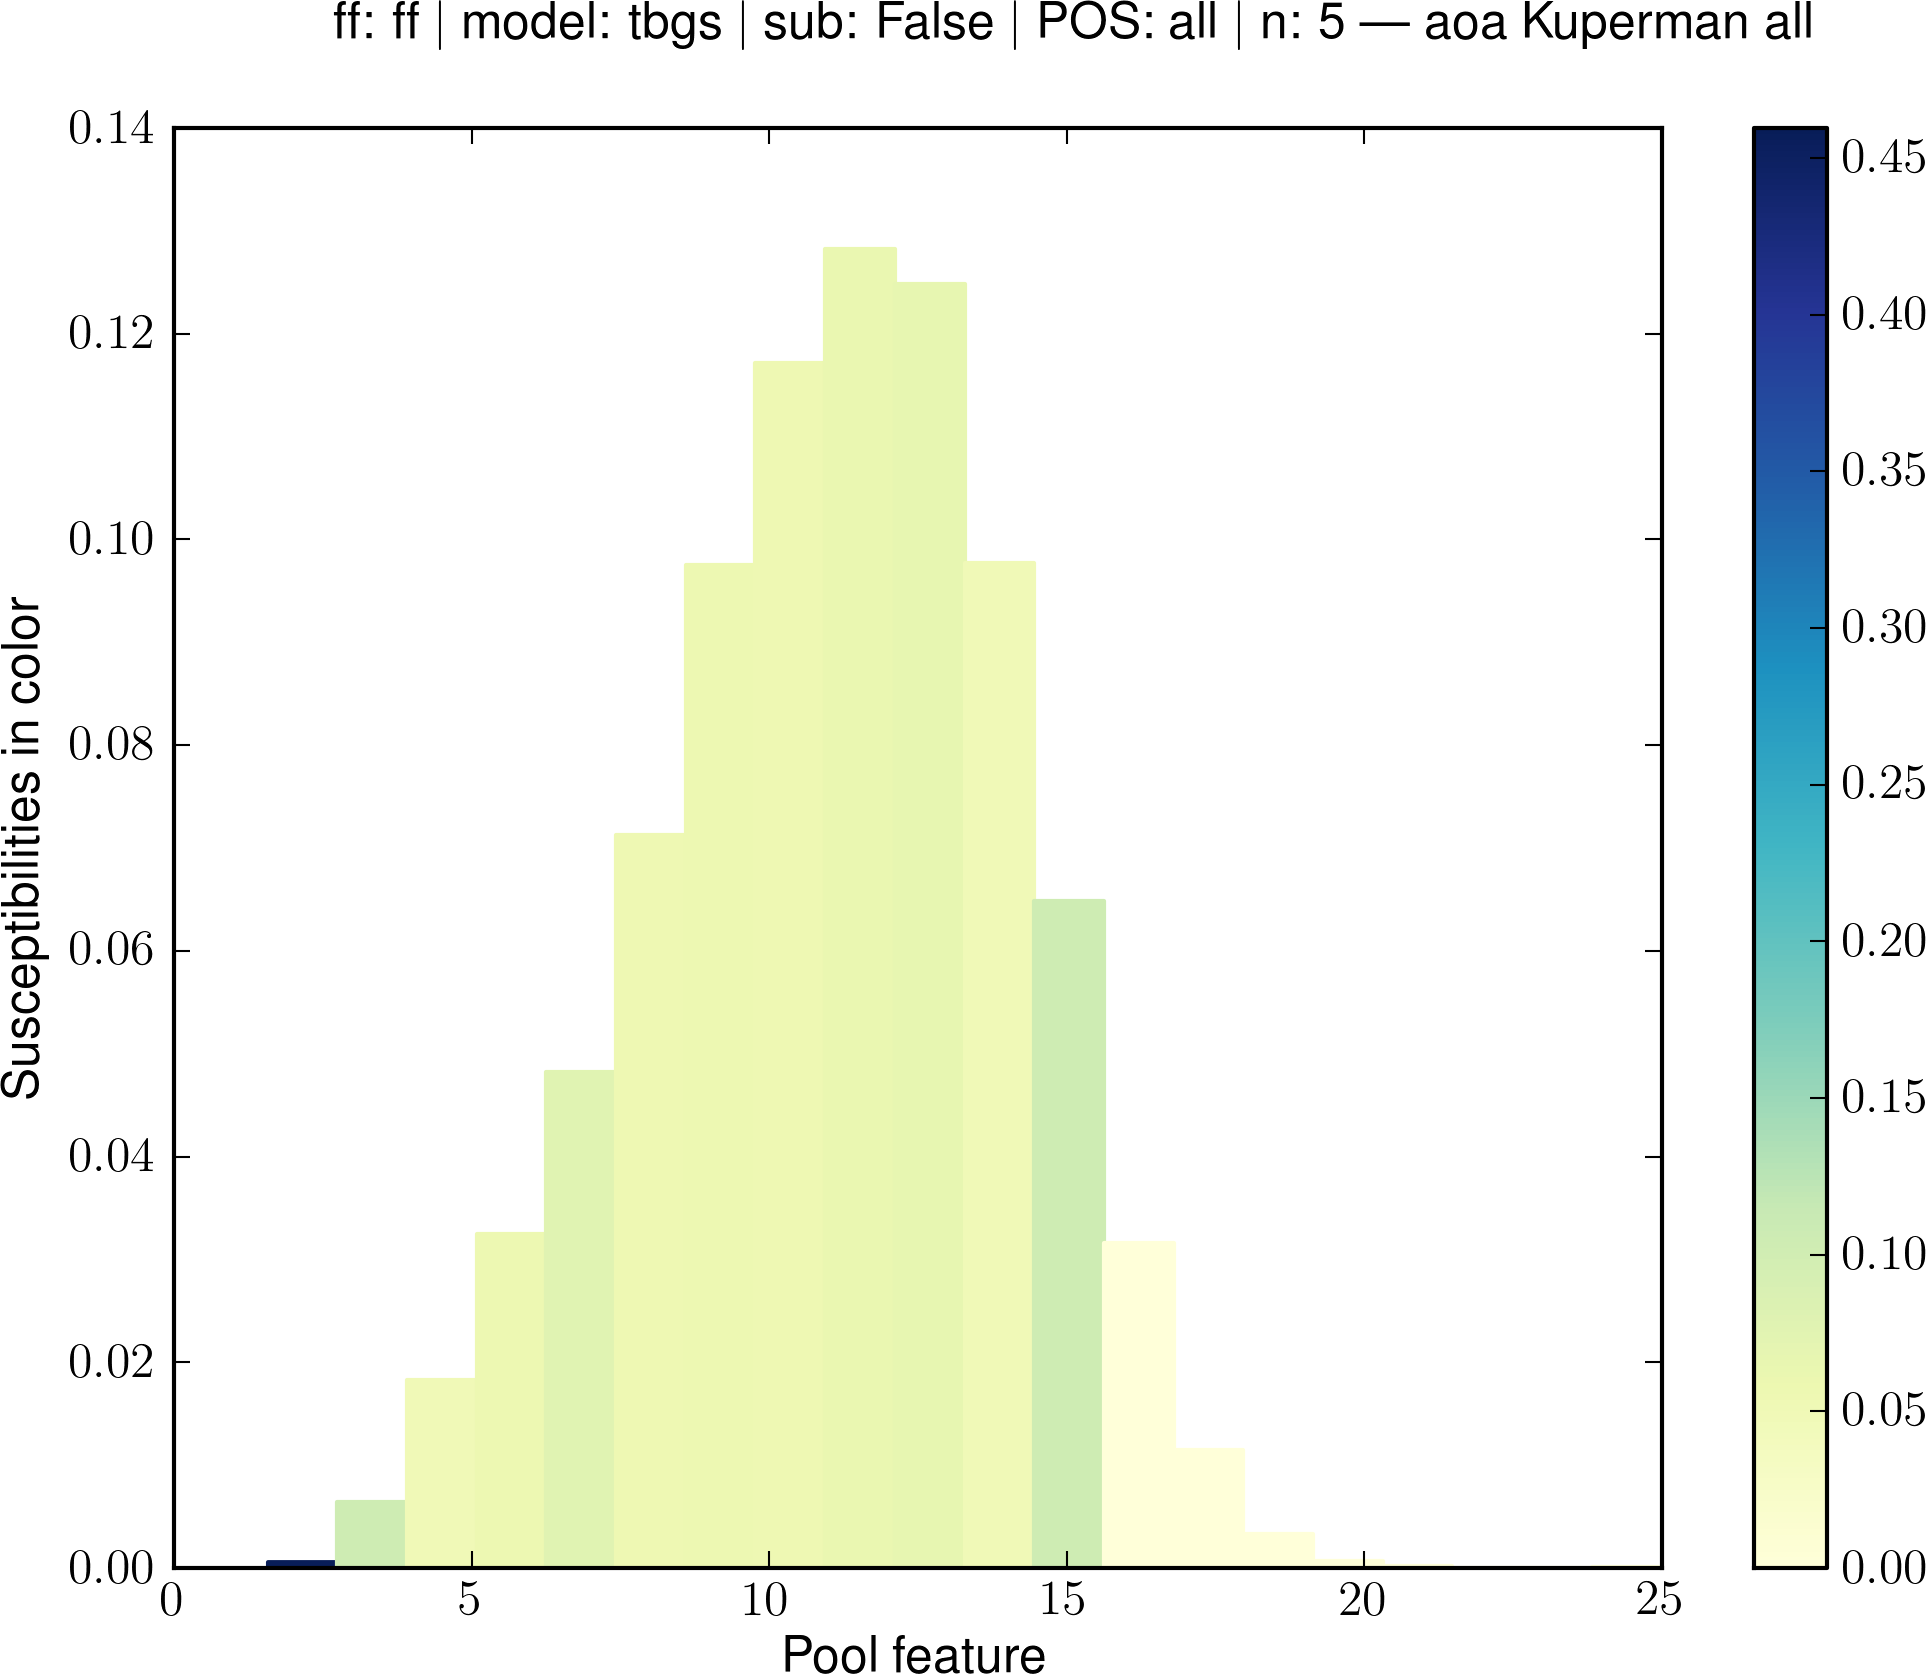
\includegraphics[width=0.3\textwidth]{images/Fff_Mtbgs_Sno_Pall_N5_aoa-Kuperman-all_suscept.png}
		\label{fig:aoa-suscept}
	}
	~
	\subfloat[][Number of phonemes]{
		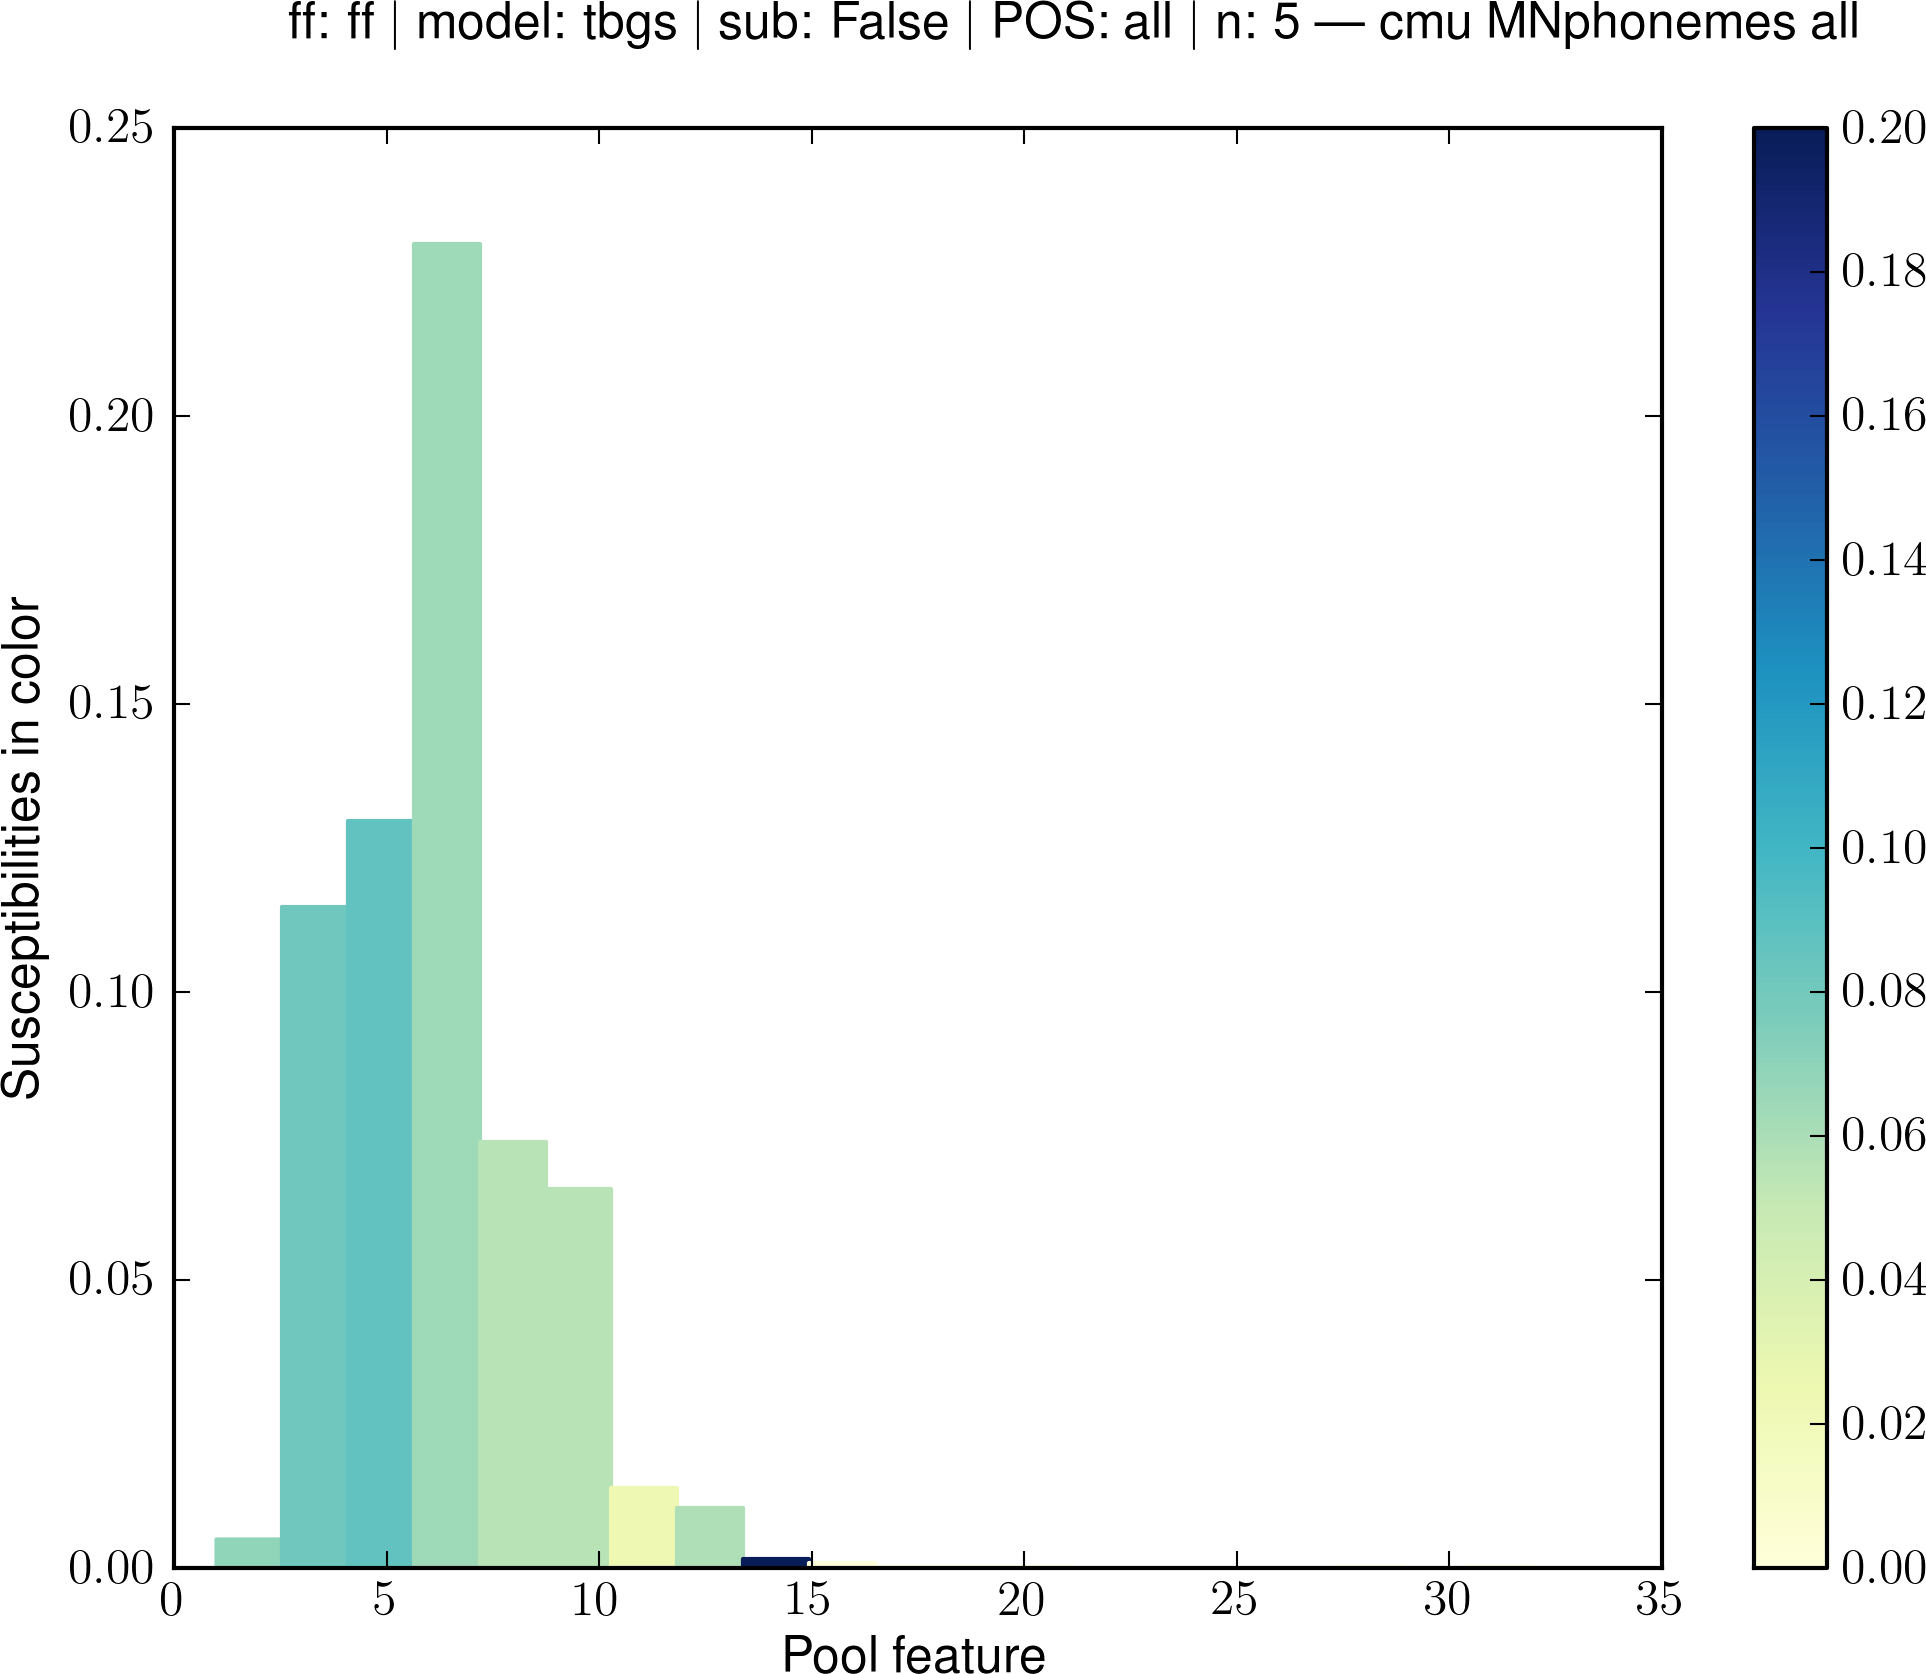
\includegraphics[width=0.3\textwidth]{images/Fff_Mtbgs_Sno_Pall_N5_cmu-MNphonemes-all_suscept.png}
		\label{fig:MNphonemes-suscept}
	}
	\caption{Susceptibility values in color over the histograms of feature values}
\end{figure*}


\begin{figure*}[!th]
	\centering
	\subfloat[][Age-of-Acquisition]{
		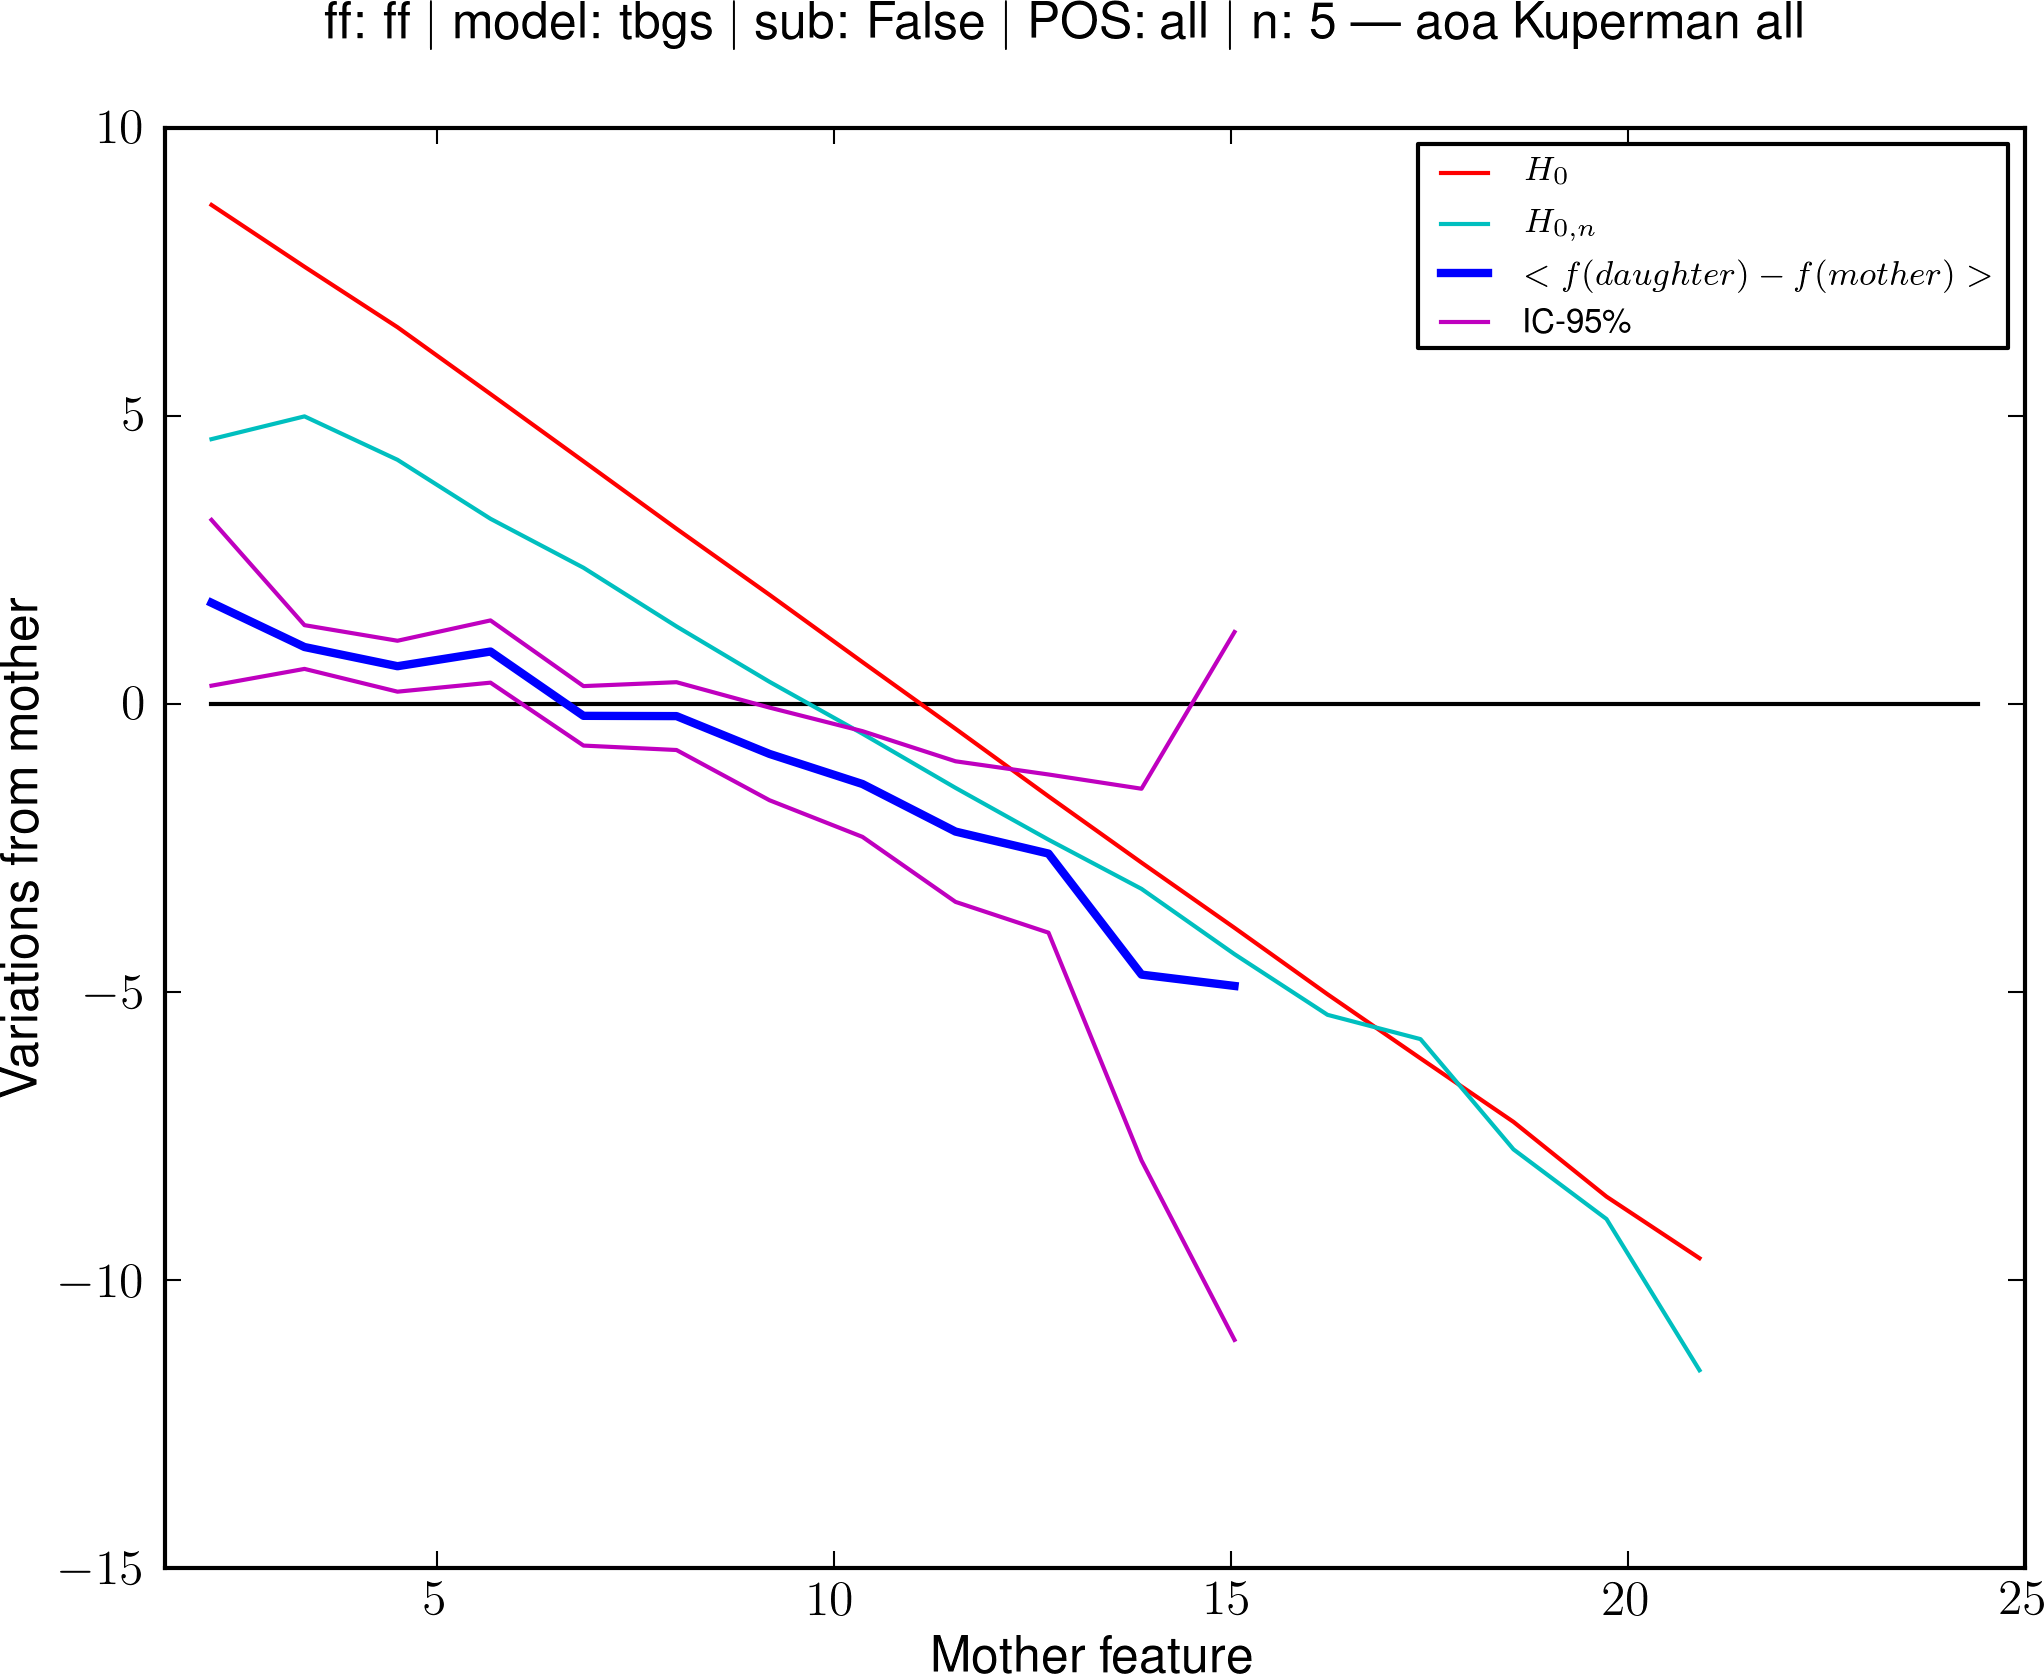
\includegraphics[width=0.3\textwidth]{images/Fff_Mtbgs_Sno_Pall_N5_aoa-Kuperman-all_absolute.png}
		\label{fig:aoa-absolute}
	}
	~
	\subfloat[][Number of phonemes]{
		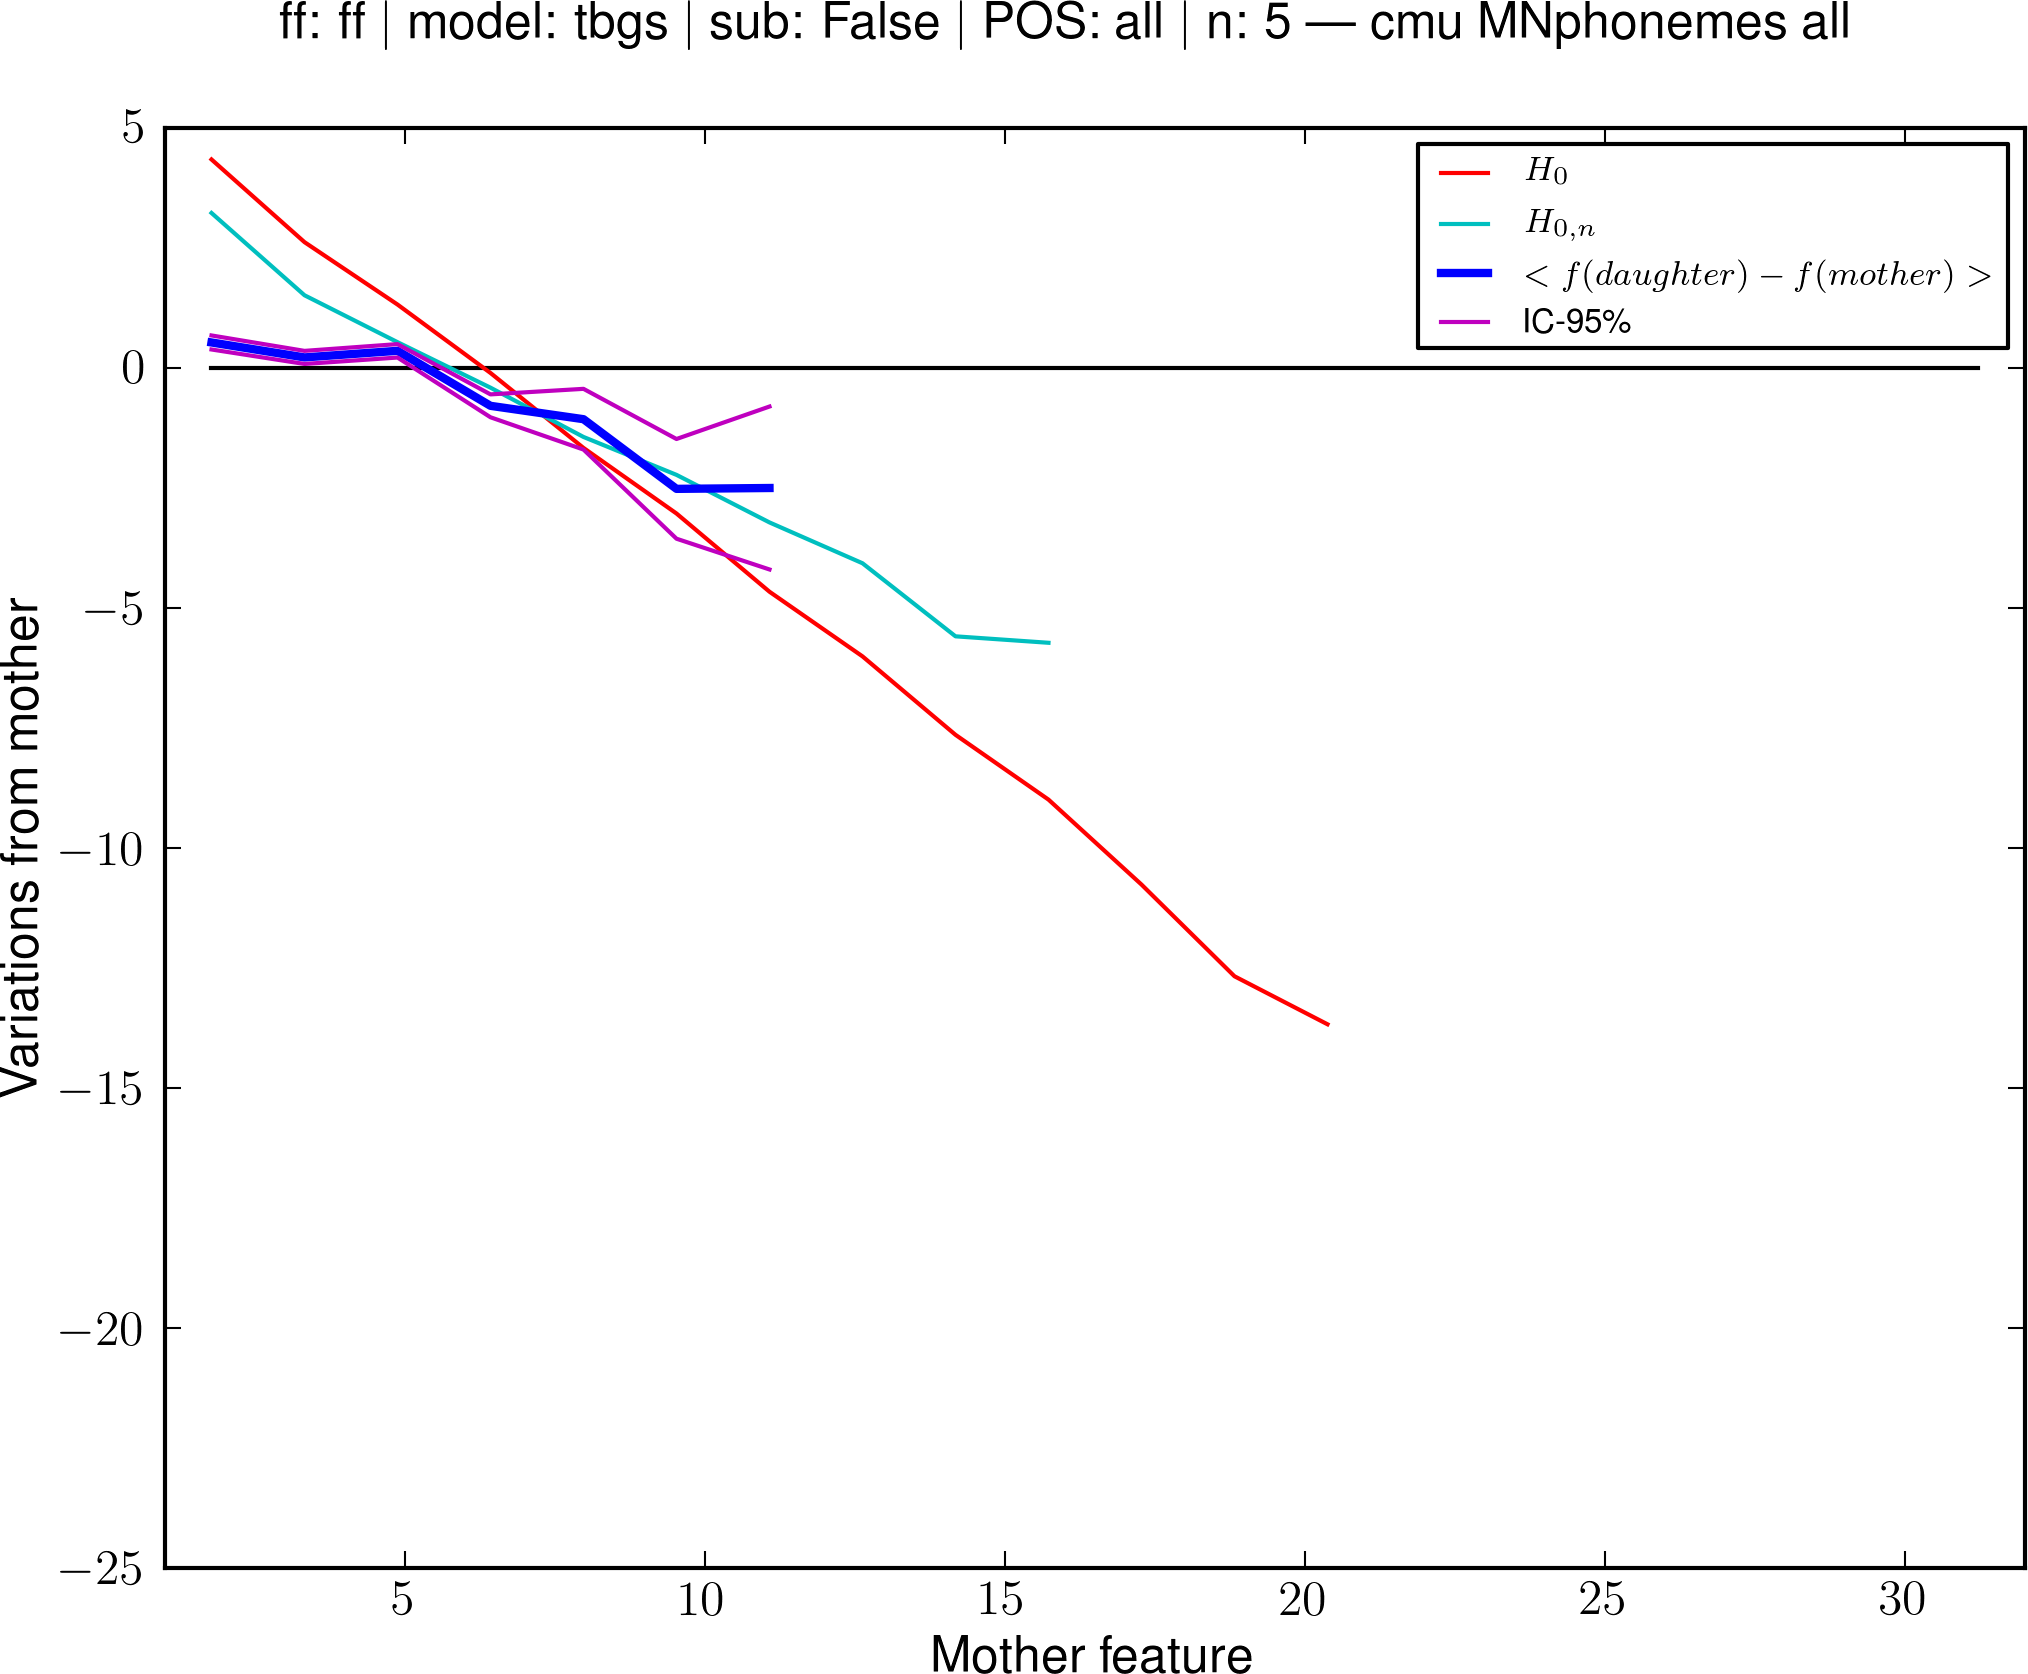
\includegraphics[width=0.3\textwidth]{images/Fff_Mtbgs_Sno_Pall_N5_cmu-MNphonemes-all_absolute.png}
		\label{fig:MNphonemes-absolute}
	}
	\caption{Variations of features, with corresponding values under $\mathcal{H}_0$ and $\mathcal{H}_{0,n}$}
\end{figure*}


\subsection{Epidemiological setting}

\TB{Secondly, and coming back to our primary goal of providing a first empirical testing means for epidemiological models of culture, we added to these two features a number of more abstract properties computed from the Free Association norms used by \citet{Griffiths07}: namely, the PageRank, betweenness coefficient and clustering coefficient of the words.} \rk{repetition}


These new features are classical measures for network-related matters, but --~to our knowledge~-- have seldom been applied to word characterization. They are only a few among many other features that can be used to characterize words based on the network they form (be it the Free Association norms network, another semantic network, or even a phonological network). We consider the complete set of these features (which includes the two mentioned in the previous section, the new network-based ones, as well as any other network-based feature one can compute) as traits characterizing words in an empirical epidemiological evolution of quotes. The benefit we get from measuring the evolution of such features is in how we can use this information to falsify epidemiological culture models. Indeed, in such a setting the information on how a feature is modified upon substitution (detailed to the individual feature value) is in fact a \emph{fitness landscape} for that particular feature. This fitness landscape can in turn be re-injected into epidemiological models to see if those models account for the empirical distribution of quotes, their life-span and relative success. The data for PageRank, betwenness coefficient and clustering coefficient are shown in figures \ref{fig:PR_scores-absolute}, \ref{fig:BCs-absolute} and \ref{fig:CCs-absolute}.

\rk{some talk about what this confirms in Griffith's work}


\begin{figure*}[!th]
	\centering
	\subfloat[][Log PageRank]{
		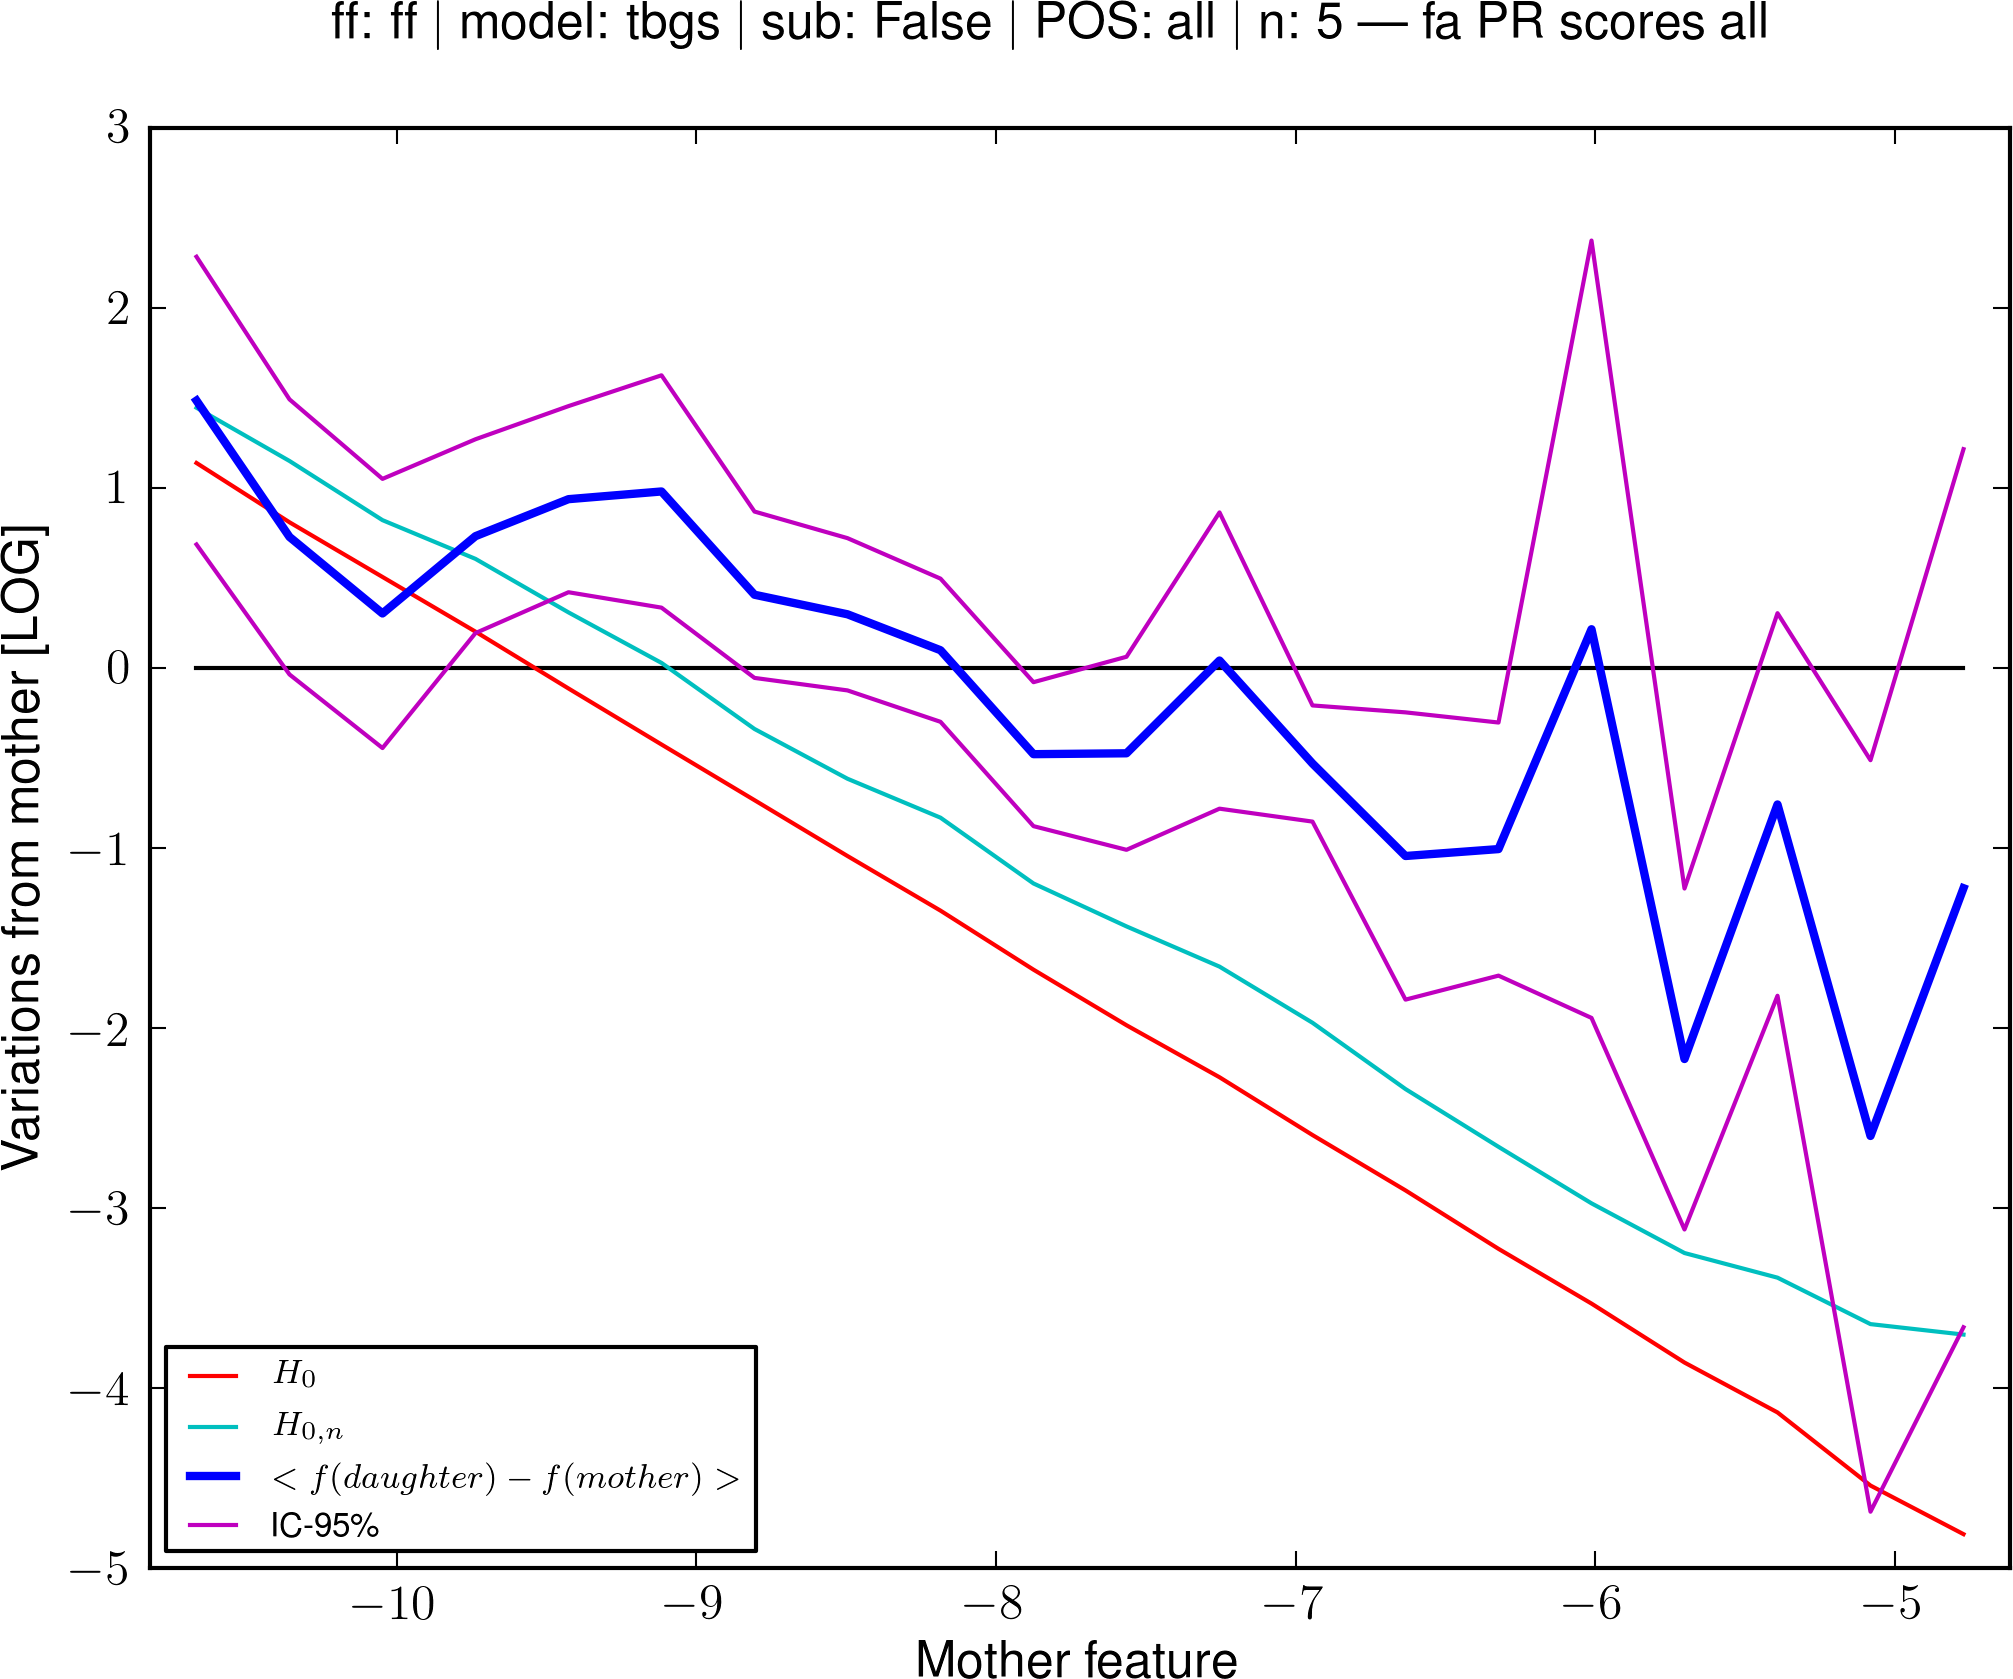
\includegraphics[width=0.3\textwidth]{images/Fff_Mtbgs_Sno_Pall_N5_fa-PR_scores-all_absolute.png}
		\label{fig:PR_scores-absolute}
	}
	~
	\subfloat[][Log Betweenness coefficient]{
		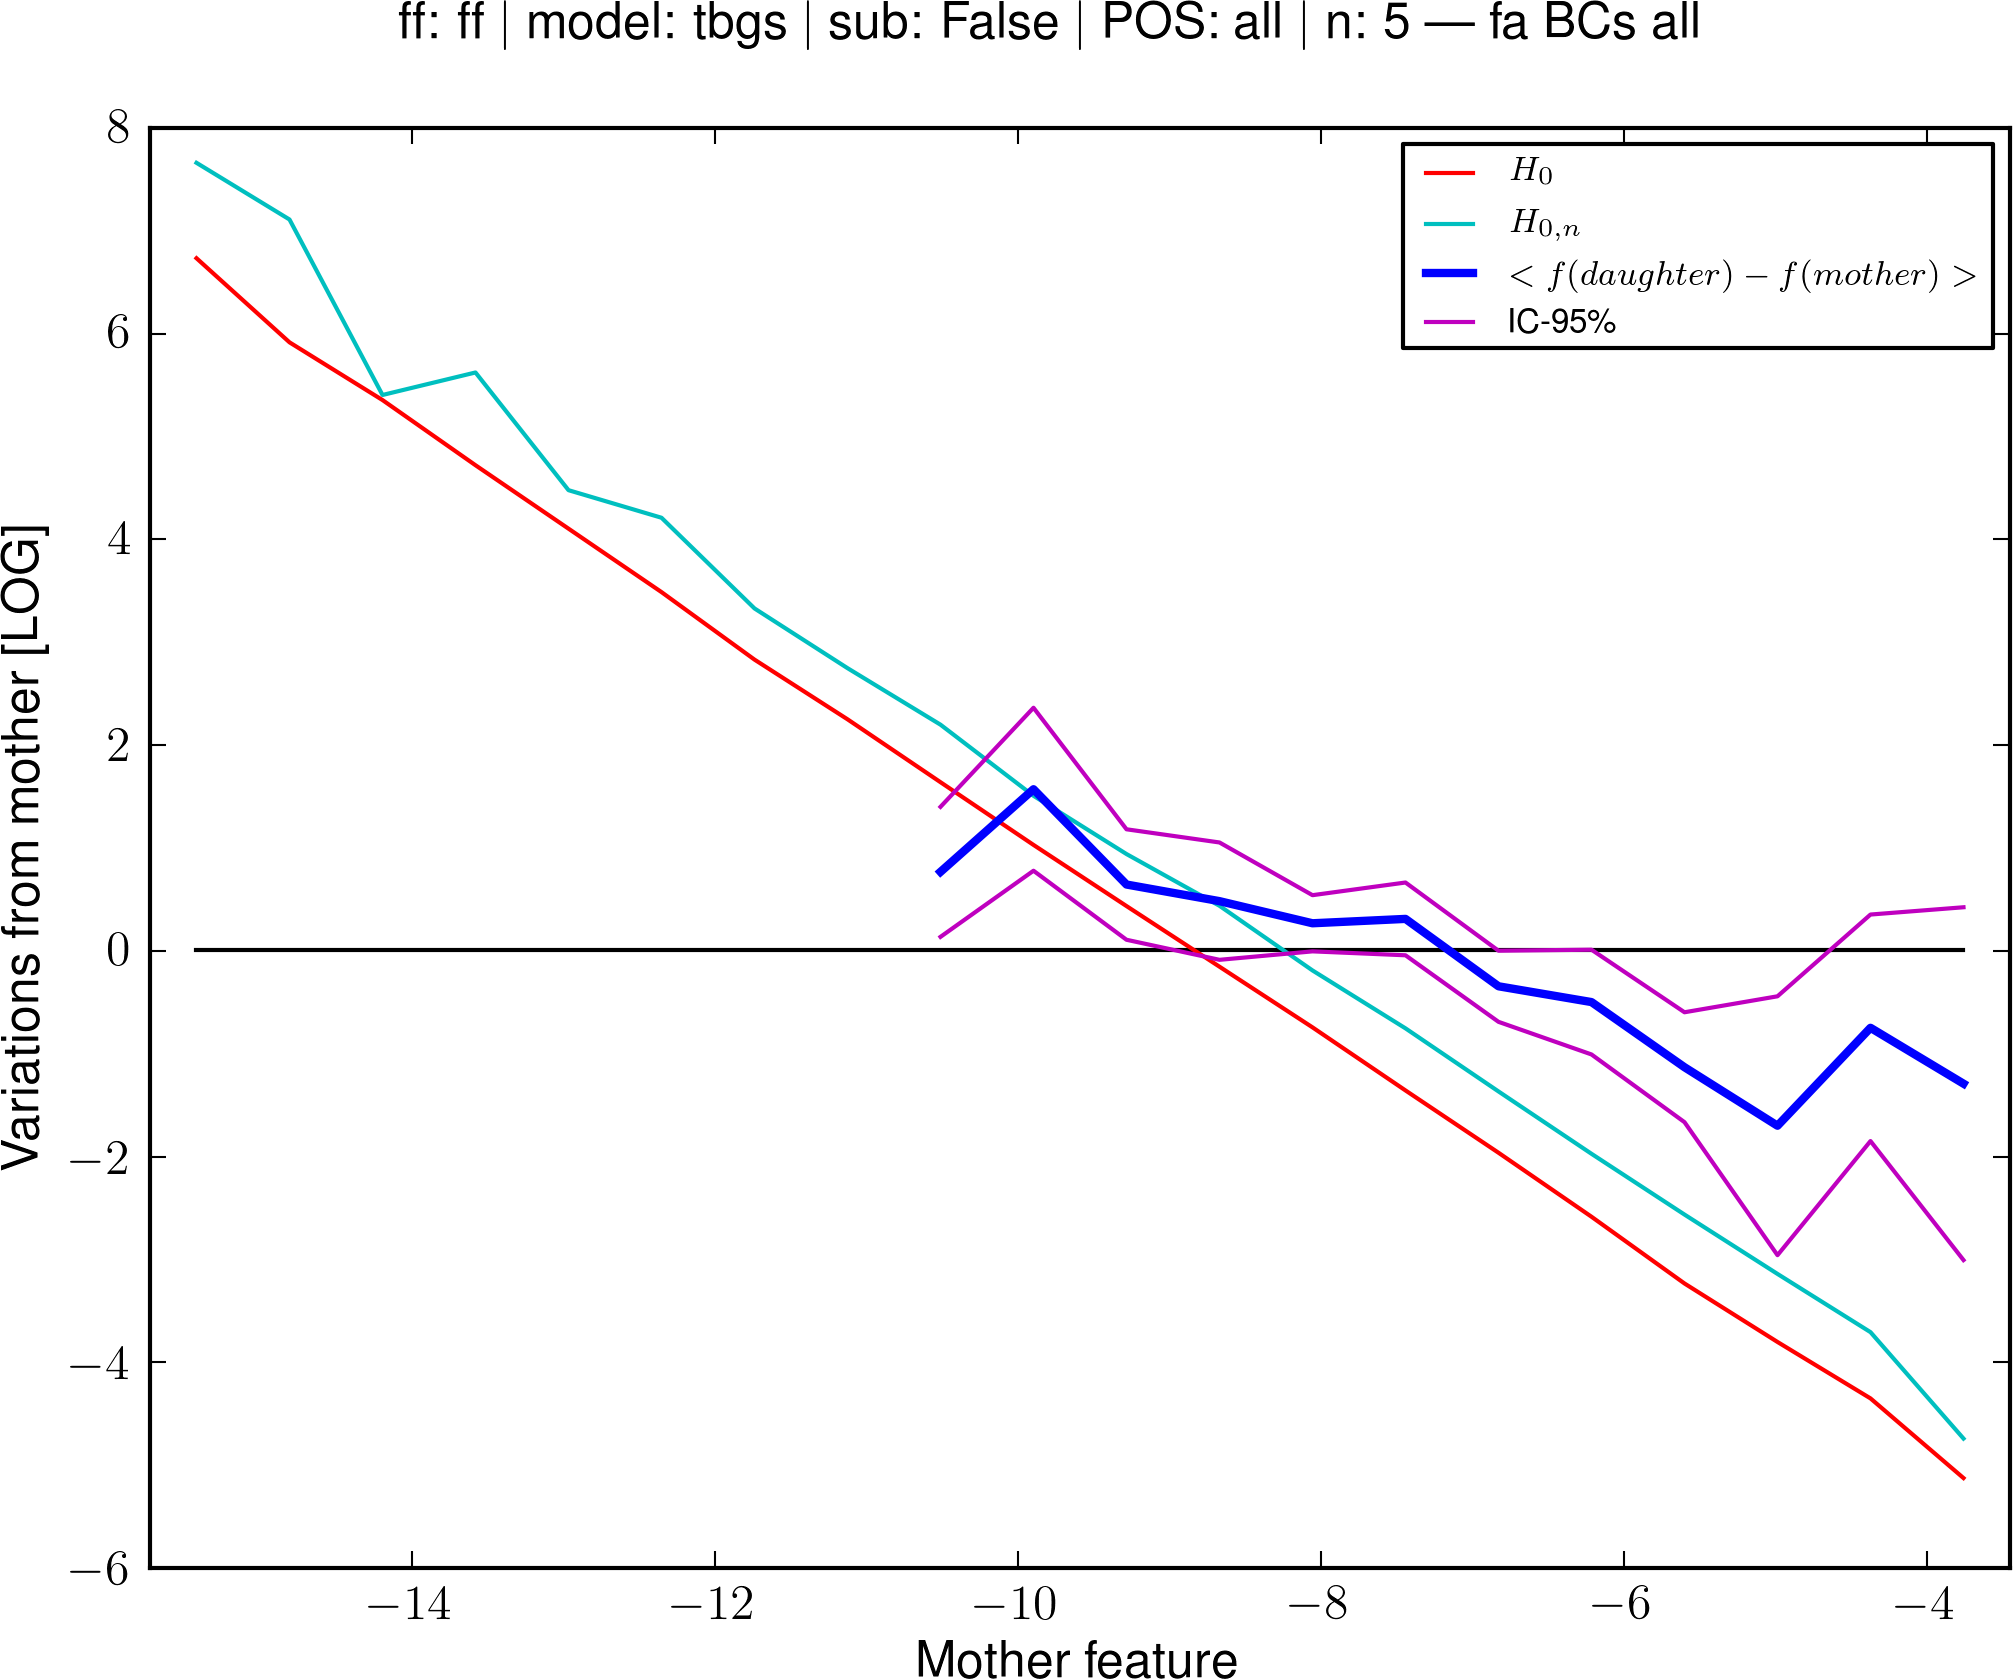
\includegraphics[width=0.3\textwidth]{images/Fff_Mtbgs_Sno_Pall_N5_fa-BCs-all_absolute.png}
		\label{fig:BCs-absolute}
	}
	~
	\subfloat[][Log Clustering coefficient]{
		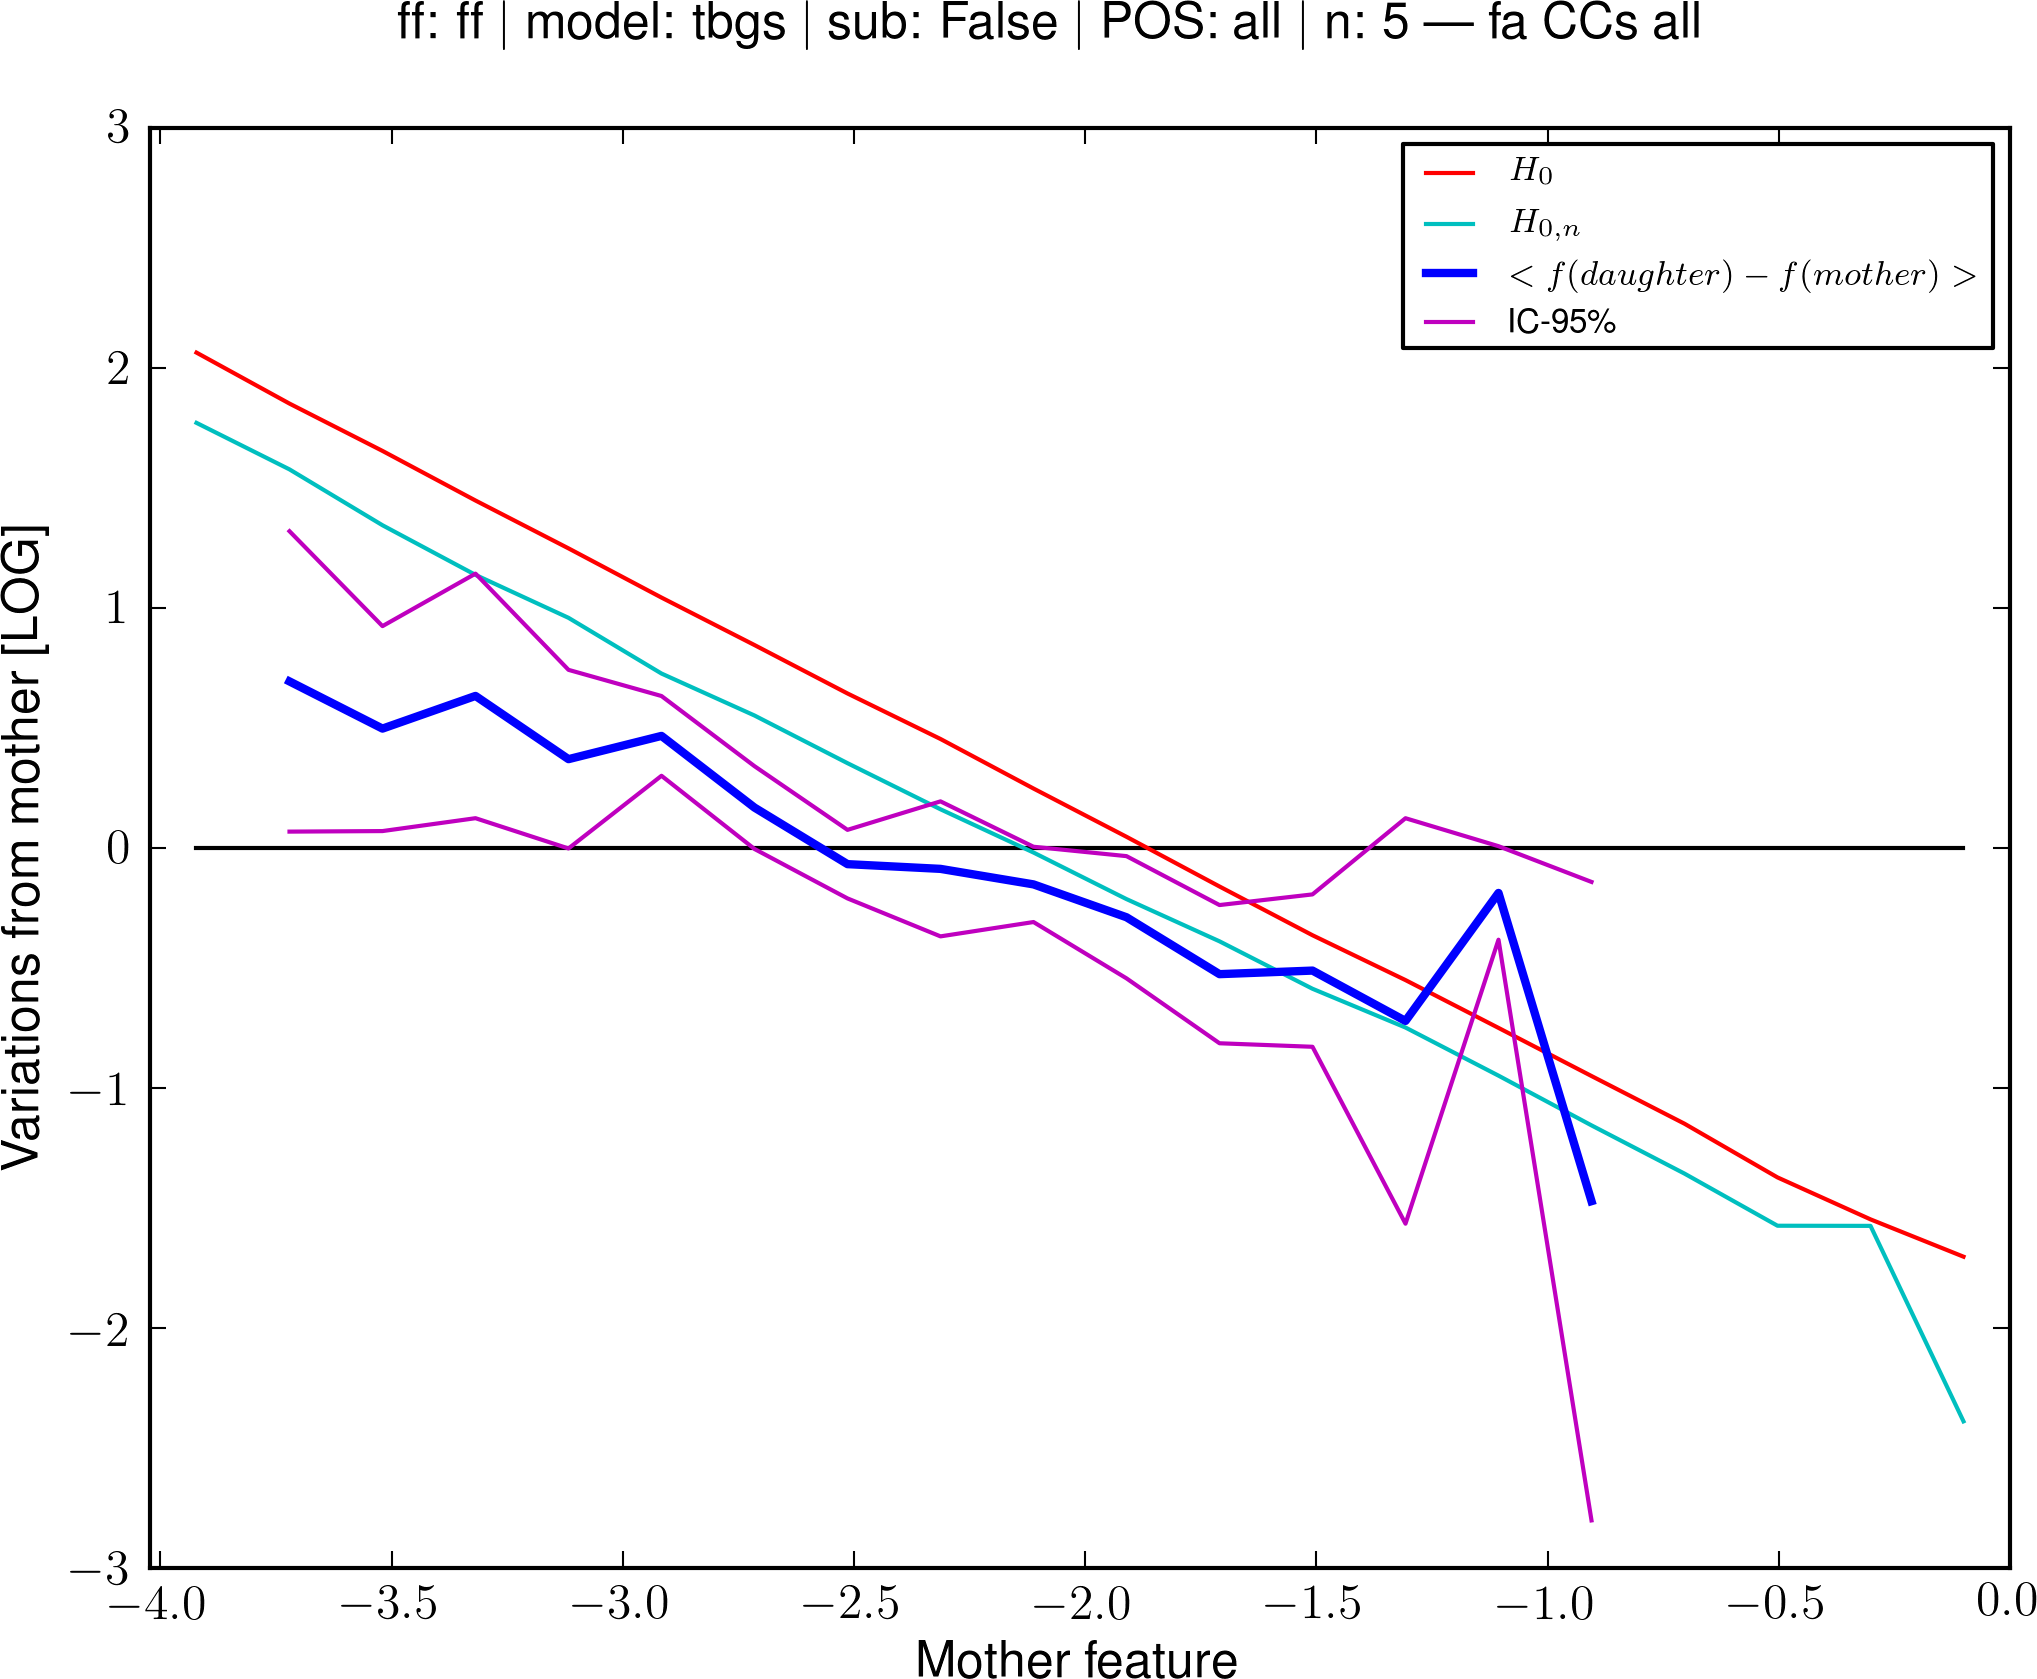
\includegraphics[width=0.3\textwidth]{images/Fff_Mtbgs_Sno_Pall_N5_fa-CCs-all_absolute.png}
		\label{fig:CCs-absolute}
	}
	\caption{Variations of features, with corresponding values under $\mathcal{H}_0$ and $\mathcal{H}_{0,n}$}
\end{figure*}


Moreover, the substitution susceptibility corresponds to a \emph{mutation probability} in this setting (shown in figures \ref{fig:PR_scores-suscept} for PageRank, \ref{fig:BCs-suscept} for betweennes coefficients, and \ref{fig:CCs-suscept} for clustering coefficient). To sum up, the data obtained here are empirical measures of (some of) the parameters of epidemiological models of cultural evolution, i.e. essential information to allow empirical testing of these models. If quotes, as a first example of cultural representation, do indeed follow epidemiological rules in their evolution, we may be able to empirically prove the validity -- or falsify -- the existing models of cultural evolution.

\rk{this is very rough and brute-like. It needs to be better presented and further developed.}


\begin{figure*}[!th]
	\centering
	\subfloat[][Log PageRank]{
		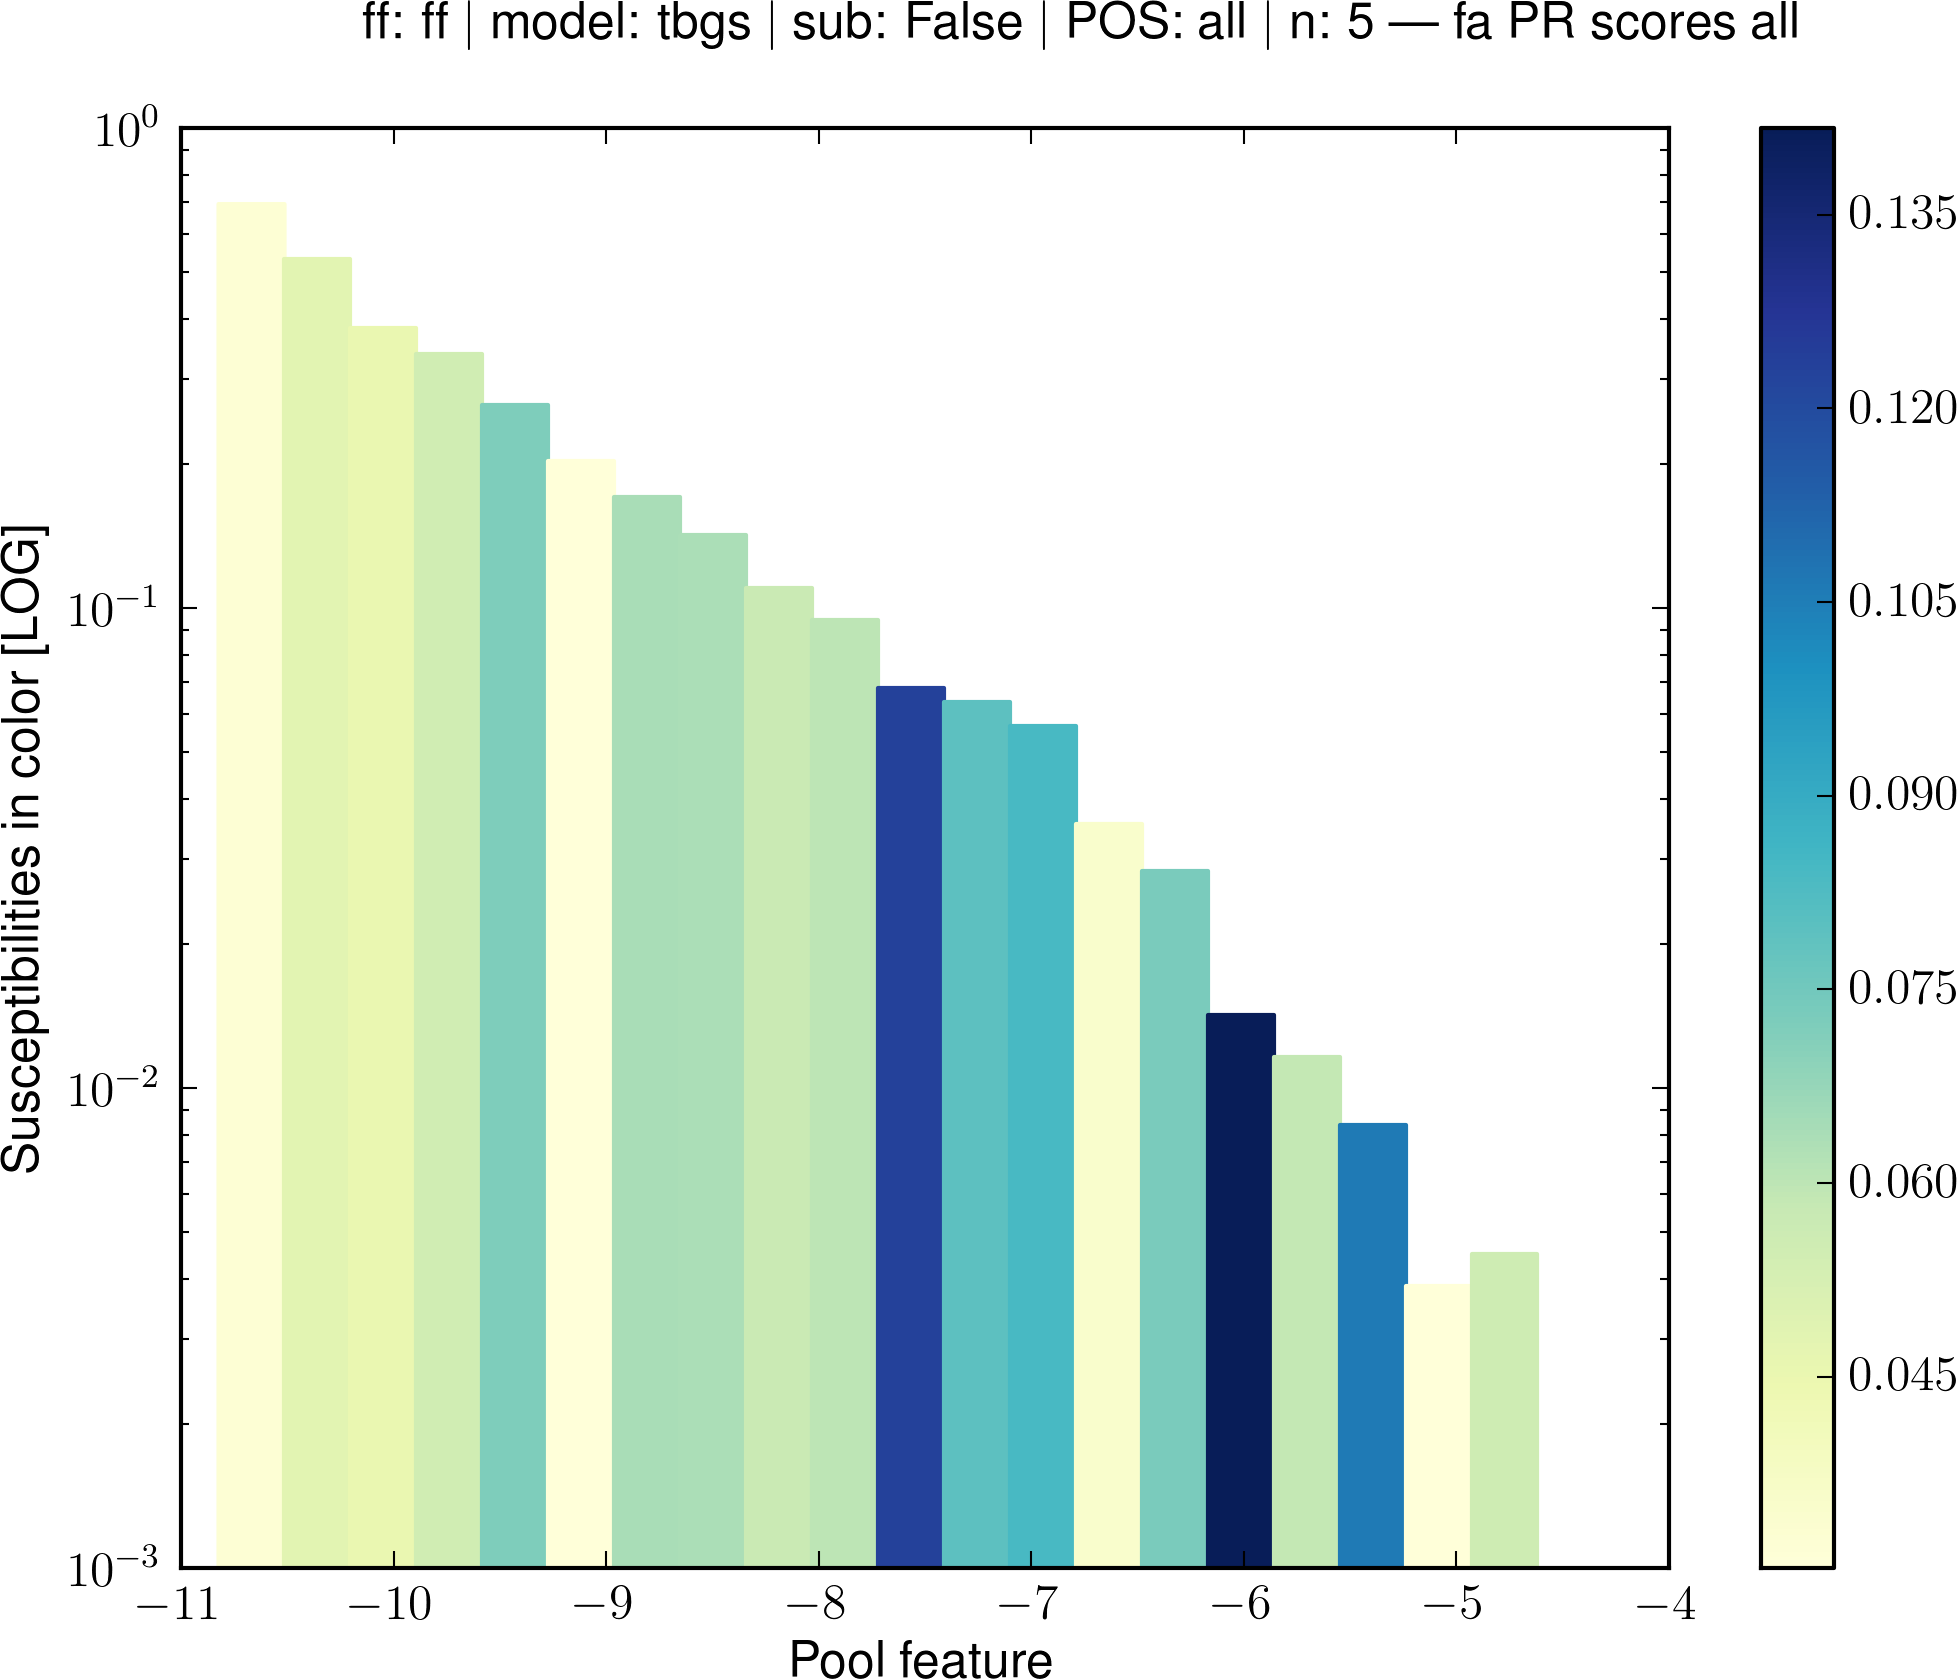
\includegraphics[width=0.3\textwidth]{images/Fff_Mtbgs_Sno_Pall_N5_fa-PR_scores-all_suscept.png}
		\label{fig:PR_scores-suscept}
	}
	~
	\subfloat[][Log Betweenness coefficient]{
		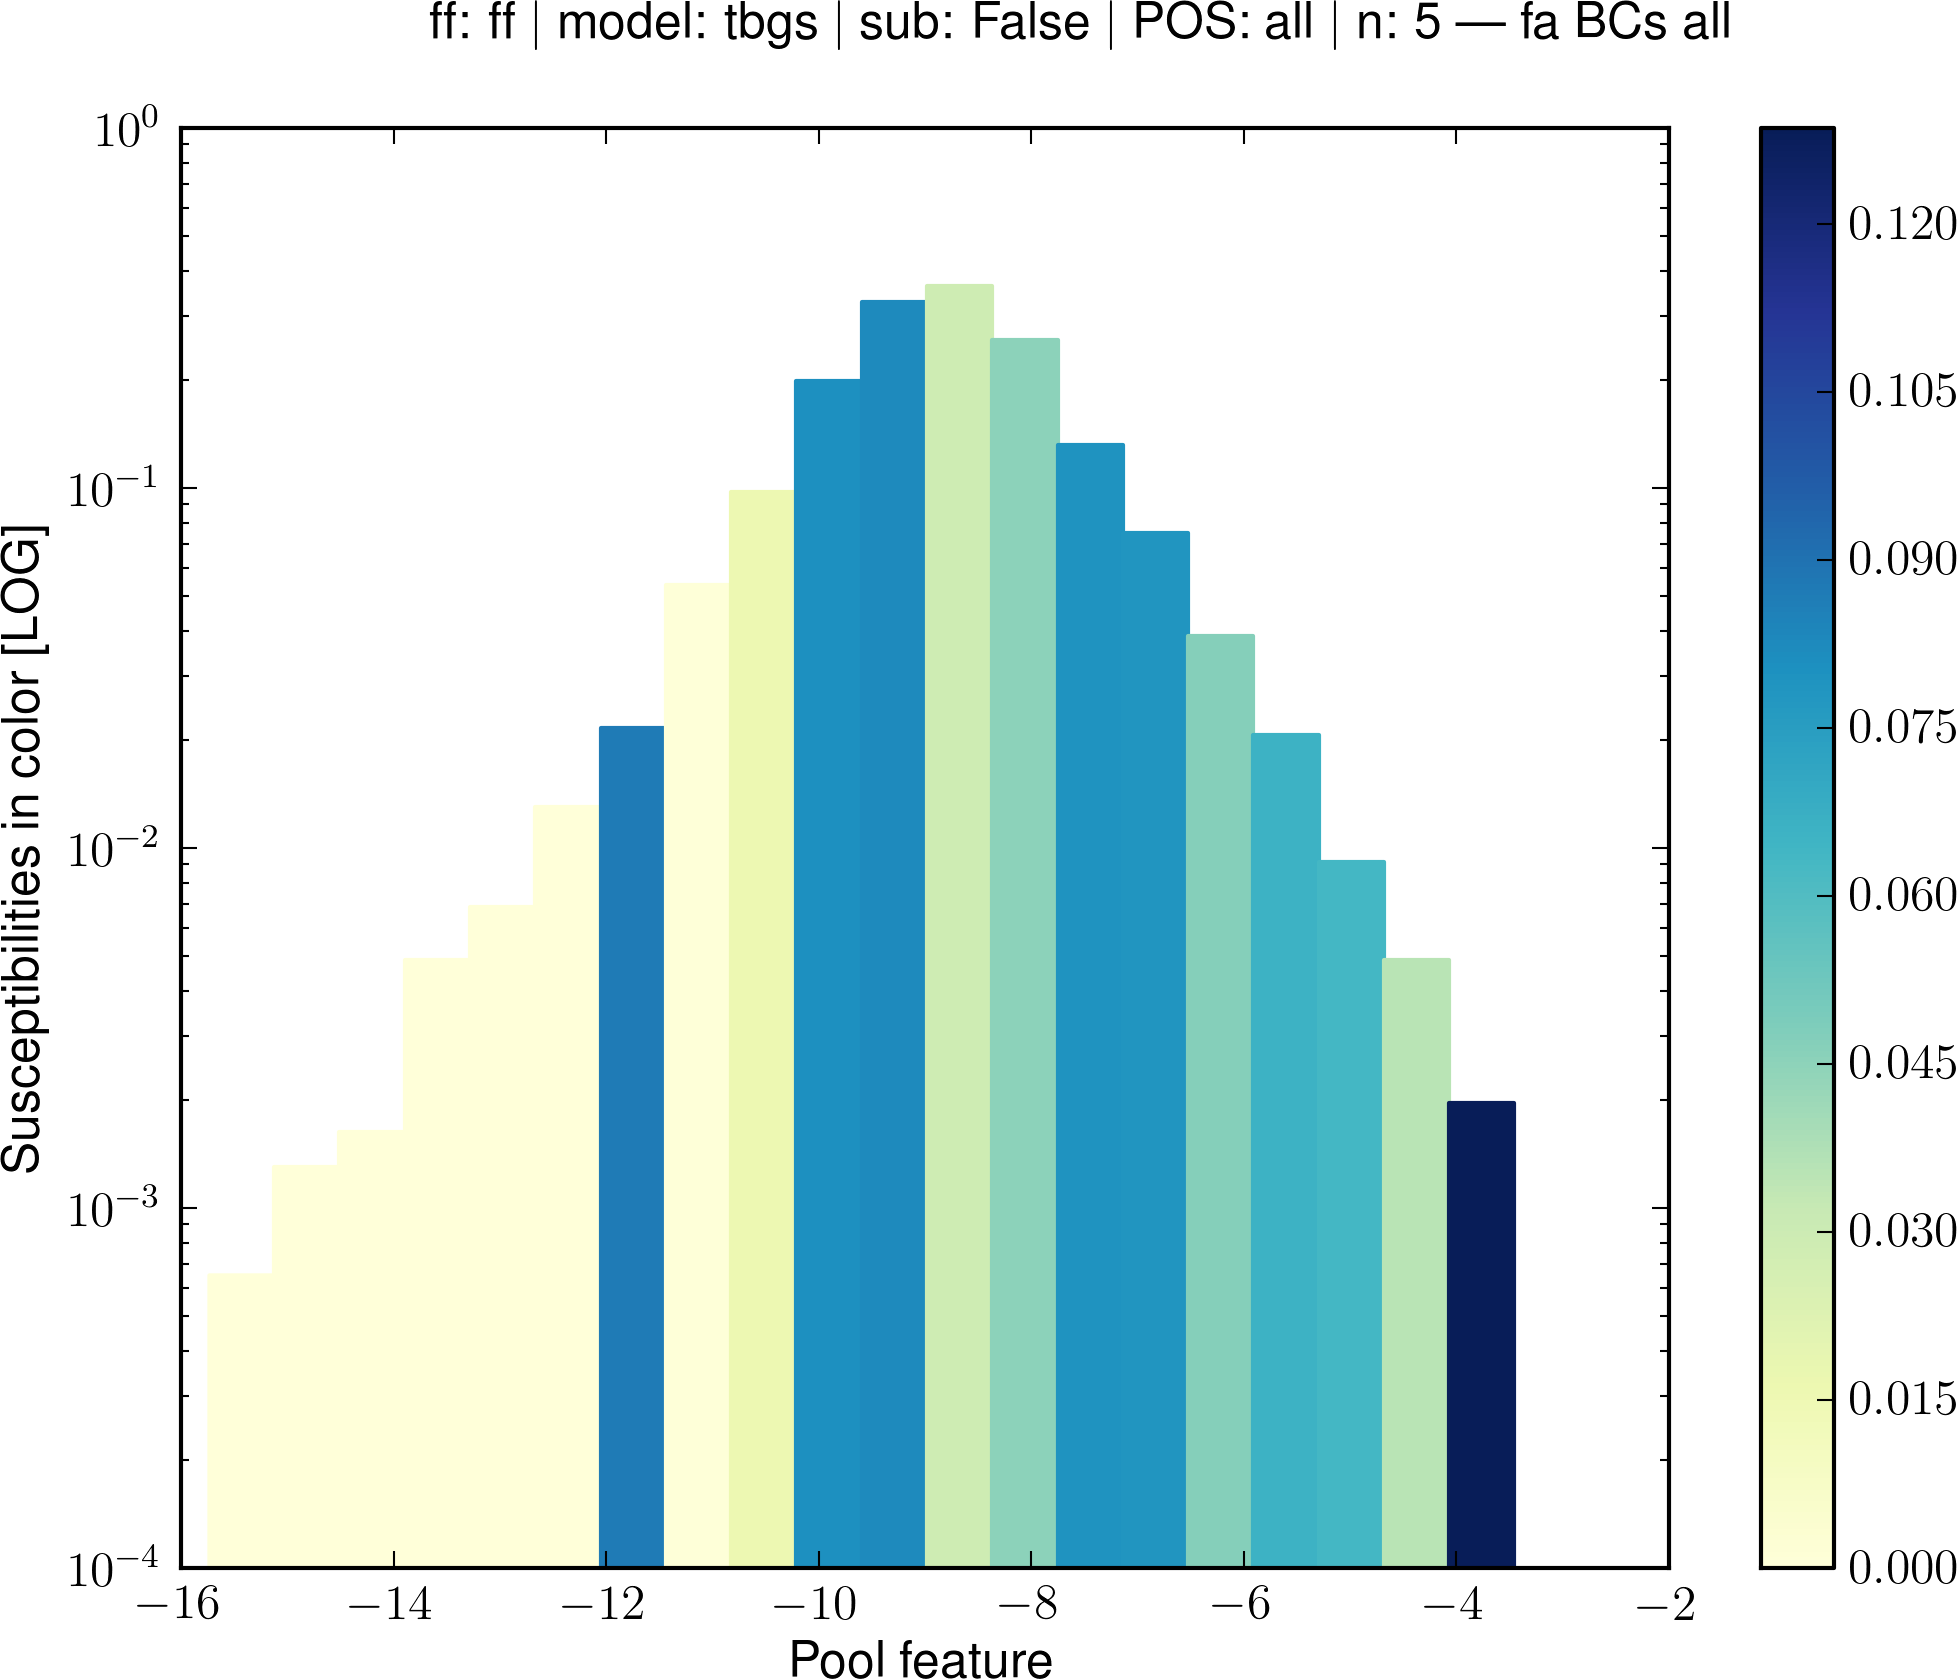
\includegraphics[width=0.3\textwidth]{images/Fff_Mtbgs_Sno_Pall_N5_fa-BCs-all_suscept.png}
		\label{fig:BCs-suscept}
	}
	~
	\subfloat[][Log Clustering coefficient]{
		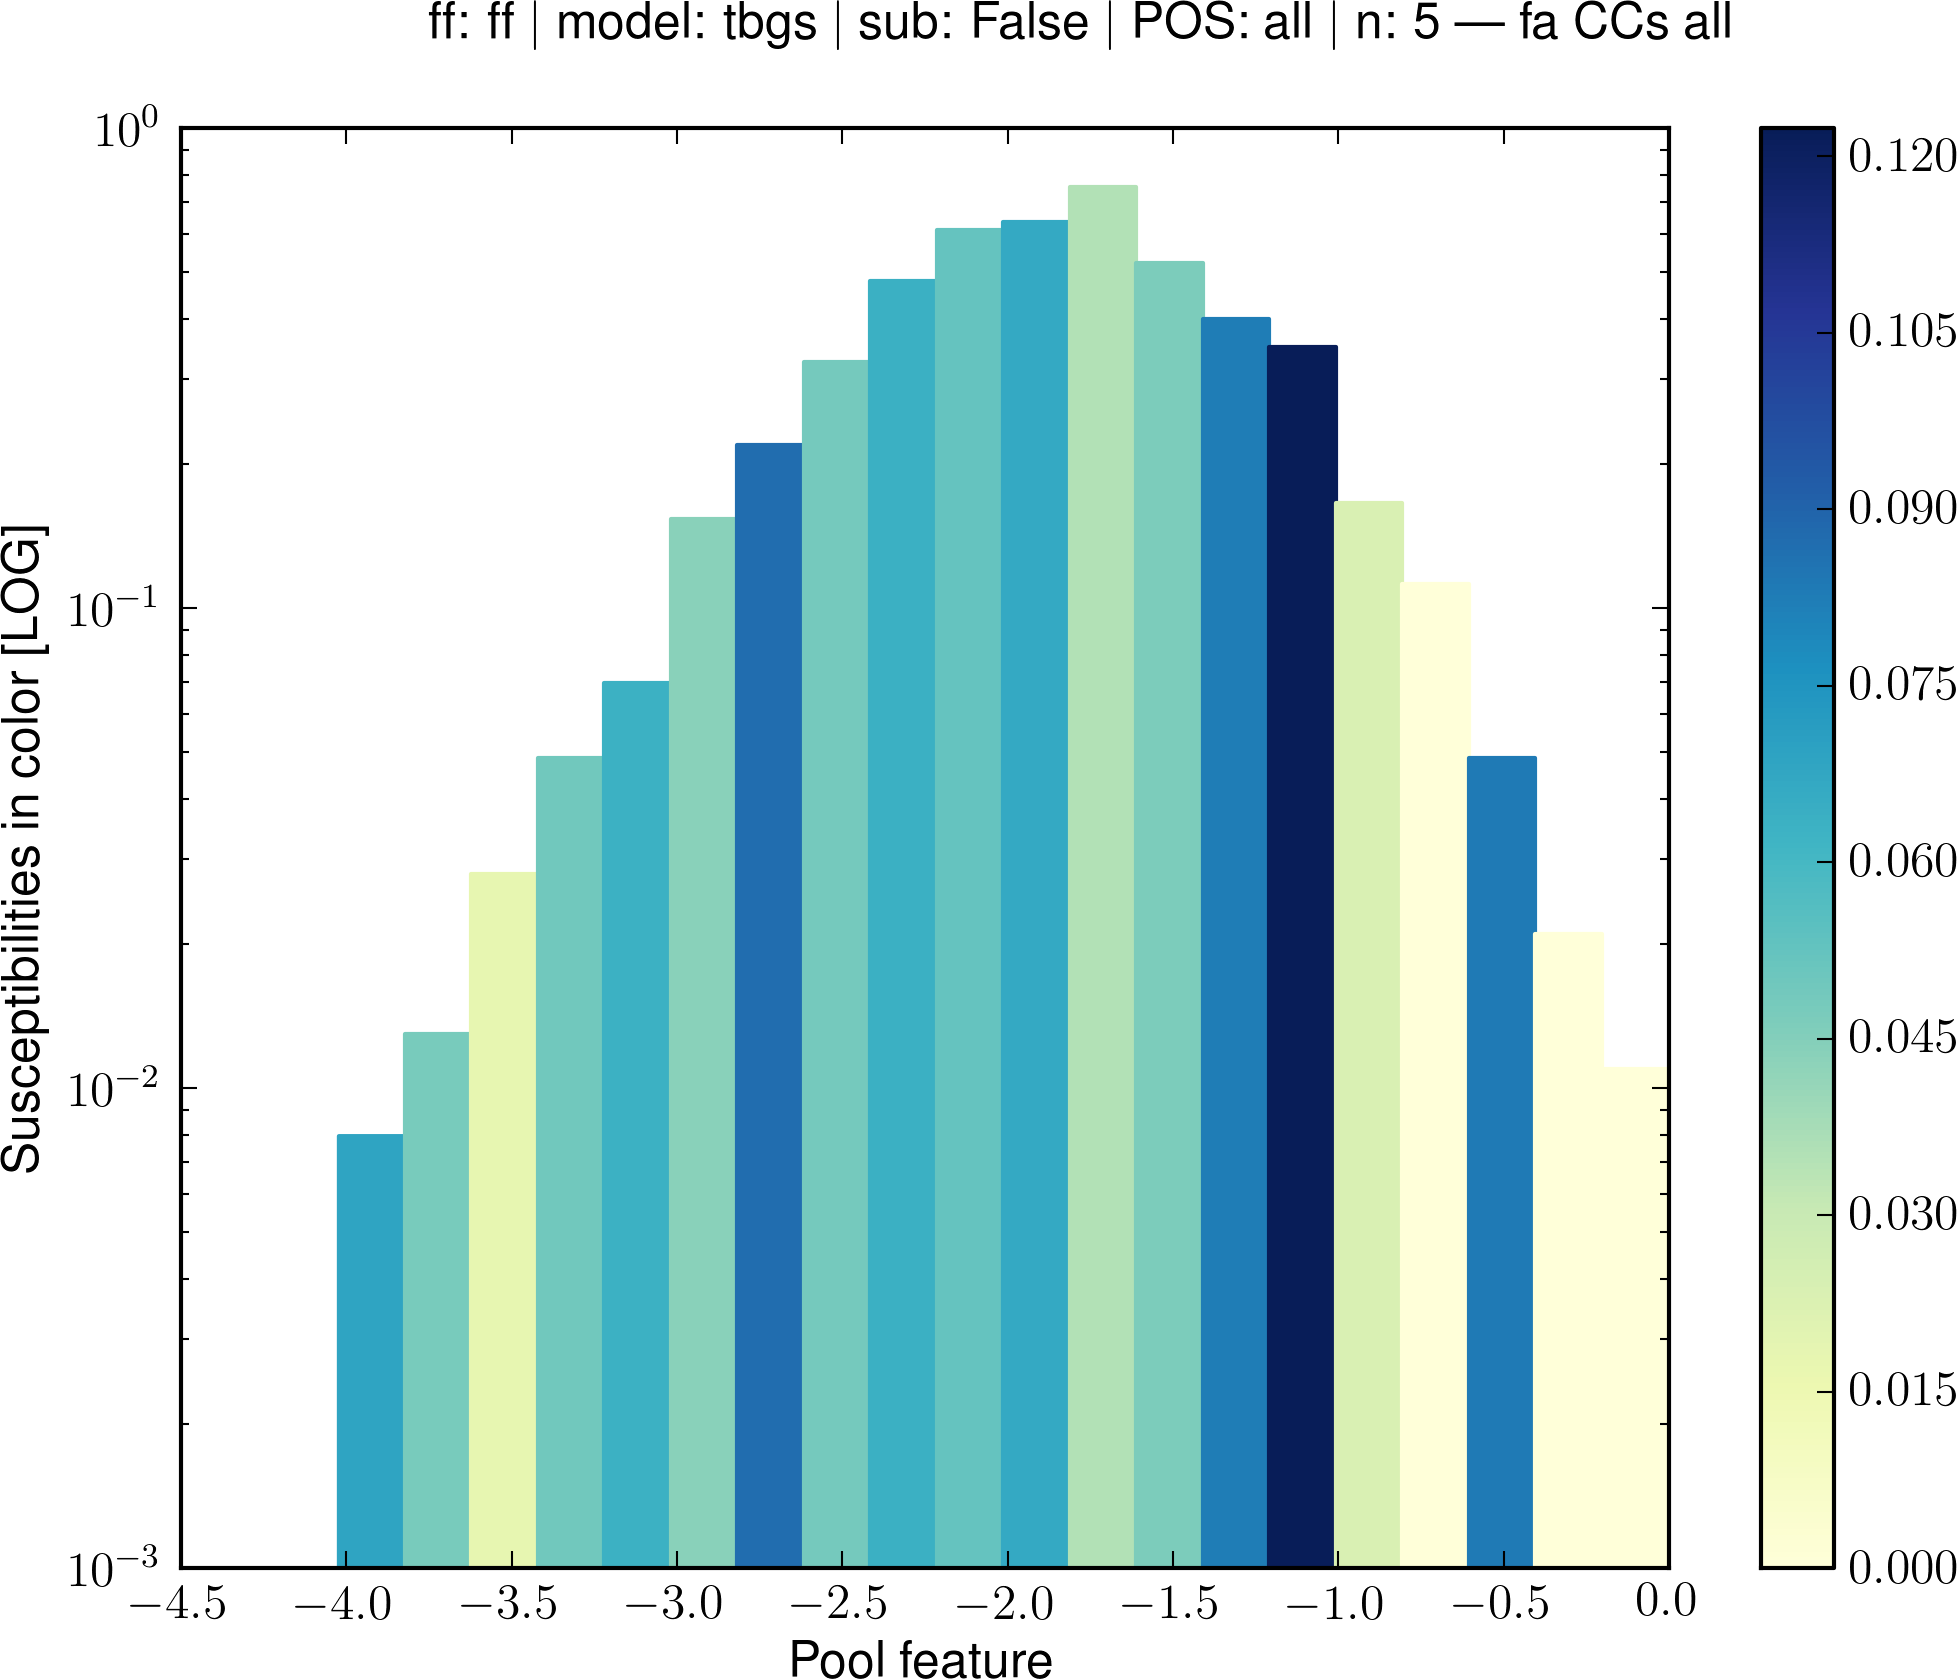
\includegraphics[width=0.3\textwidth]{images/Fff_Mtbgs_Sno_Pall_N5_fa-CCs-all_suscept.png}
		\label{fig:CCs-suscept}
	}
	\caption{Susceptibility values in color over the histograms of feature values}
\end{figure*}

%\begin{figure}[!th]
%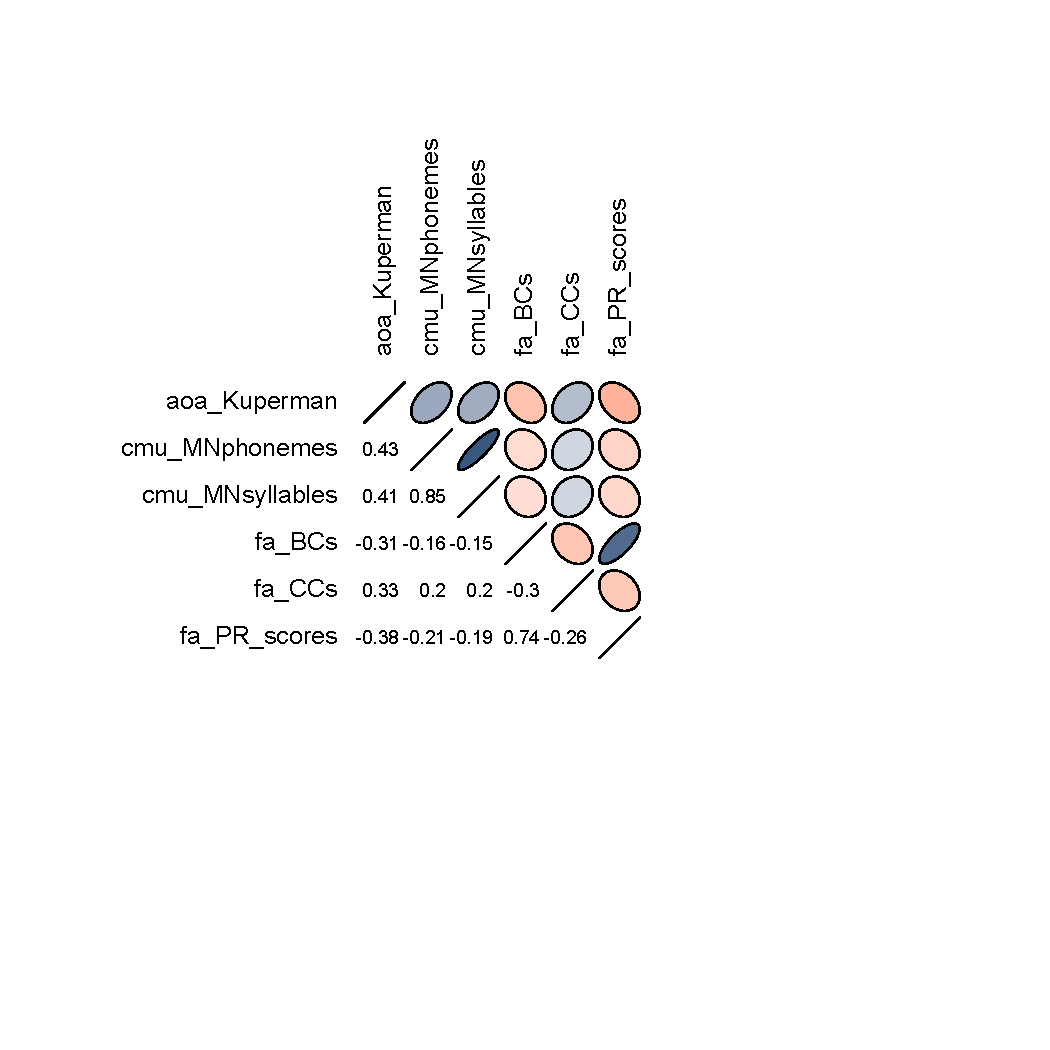
\includegraphics[width=\linewidth]{algorithms/Rplot.pdf}
%\end{figure}